% gjilguid2e.tex
% V2.0 released 1998 December 18
% V2.1 released 2003 October 7 -- Gregor Hutton, updated the web address for the style files.

%\documentclass{gji}
\documentclass[extra,mreferee]{gji}
\usepackage{timet,color}
\usepackage{graphicx}
\usepackage{amsmath}
\usepackage[urlcolor=blue,citecolor=black,linkcolor=black]{hyperref}
\usepackage{lineno}
\usepackage[inline]{trackchanges} %for better track changes. finalnew option will compile document with changes incorporated.

\linenumbers
\title[Controls on Surface Wave Overtone Interference]
  {Controls on Surface Wave Overtone Interference}
\author[Hariharan et al.]
  {Anant Hariharan$^1$, Colleen A. Dalton$^1$,  Jordyn Babikoff$^1$, G{\"o}ran Ekstr{\"o}m$^2$ \\
  $^1$ Department of Earth, Environmental, and Planetary Sciences, Brown University, Providence, RI, United States\\
  $^2$ Lamont-Doherty Earth Observatory of Columbia University, United States}

\date{Received N; in original form 2021 }
\pagerange{\pageref{firstpage}--\pageref{lastpage}}
\volume{N}
\pubyear{2021}

%\def\LaTeX{L\kern-.36em\raise.3ex\hbox{{\small A}}\kern-.15em
%    T\kern-.1667em\lower.7ex\hbox{E}\kern-.125emX}
%\def\LATeX{L\kern-.36em\raise.3ex\hbox{{\Large A}}\kern-.15em
%    T\kern-.1667em\lower.7ex\hbox{E}\kern-.125emX}
% Authors with AMS fonts and mssymb.tex can comment out the following
% line to get the correct symbol for Geophysical Journal International.
\let\leqslant=\leq

\newtheorem{theorem}{Theorem}[section]

\begin{document}

\label{firstpage}

\maketitle


\begin{summary}
Measurements of fundamental-mode (FM) surface waves along the minor arc are impacted by overtone interference. This interference is primarily due to major-arc overtones for Rayleigh waves and minor-arc overtones for Love waves. In both cases, interference contaminates measurements of phase and amplitude and can introduce bias in seismic images. Here, we use synthetic seismograms computed via normal mode summation to probe how interference can vary as a function of the surface-wave group velocities, source mechanism and depth, which control the relative excitation of the FM and overtones, and period. By comparing seismograms that include all overtones to those that include only the FM, we can quantify the interference, i.e., how the presence of the overtones perturbs the FM phase and amplitude. We compare the strength of this interference to calculations of excitation of the overtones and FM. We show that these calculations explain well the varying strength of interference for different source mechanisms and depths. Notably, these calculations illuminate source depths where Love wave overtone excitation is quite low and therefore interference is unusually weak, and depths where Rayleigh wave FM excitation is low and therefore interference is unusually strong. Our analysis also reinforces the dependence of the interference on the FM and overtone group velocities. For Love waves, this results in weak minor-arc overtone interference at long periods and, for continental paths, short periods. For Rayleigh waves, the differing overtone and FM group velocities and the relative excitation of the overtones and FM explain rapid variations in the strength of Rayleigh wave major-arc overtone interference as a function of epicentral distance. We then show that real data are affected by the relative excitation of the FM and overtones. We find that errors in Rayleigh wave phase velocities across USArray are larger when the ratios of overtone to FM excitation are larger. We also find a dependence of phase velocity error on excitation ratio for Love waves, and identify the presence of major-arc overtone interference in Love wave measurements. Our results highlight opportunities for more nuanced quality control of surface-wave measurements. The relative excitation ratio of the overtones and FM may be a better criterion for event selection than source depth, allowing deeper events that well excite FMs to be included and shallower events with large overtone excitation to be excluded. This would allow larger and cleaner data sets that will increase the precision of seismic images.
\end{summary}

\begin{keywords}
Surface waves and free oscillations, Seismic tomography, Theoretical seismology
\end{keywords}

\section{Introduction}
Measurements of the phase and amplitude of fundamental-mode (FM) Rayleigh  and Love waves are critical to our understanding of the seismic structure of the upper mantle since both types of surface waves have a period-dependent sensitivity to shear velocity \citep[e.g.][]{nettles2008radially}. Secondary observables calculated from these surface-wave measurements include phase velocities \citep[e.g.][]{lin2011helmholtz, eddy2018age}, H/V ratios \citep[e.g.][]{tanimoto2008zh}, and attenuation \citep[e.g.][]{dalton2006global}, all of which inform models of the Earth's physical, chemical, and anisotropic properties \citep[e.g.][]{dalton2017thermal,altoe2020thermo,russell2019high}. Improving the quality and quantity of surface-wave observations thus has the potential to augment the accuracy and resolution with which we can image the interior of the Earth.

It is well established that measurements of FM surface-wave phase and amplitude along the minor arc can be biased by higher-mode, or overtone, interference, especially for FM Love waves. This interference is manifest as oscillations in phase and amplitude as a function of epicentral distance, which can then propagate into secondary observables such as phase velocity \citep[e.g.][]{thatcher1969higher,foster2014overtone,hariharan2020evidence}. Interference thus poses a challenge to obtaining accurate seismic images, and it is a particular challenge for array-based studies that seek high-resolution models, as demonstrated by  \citet{foster2014overtone} and \citet{hariharan2020evidence}. 

Overtone interference with FM Love waves arises because of the closeness of FM and overtone group velocity, especially at periods $<$ 100 s and for propagation through an oceanic-type velocity model with a well defined low-velocity zone (Fig. 1a,b). Early studies described the oscillatory character of Love wave overtone interference \citep{thatcher1969higher,boore1969effect}, showed it was a particular problem in oceanic settings \citep{thatcher1969higher,yoshida19831}, and modeled the wavefield as interference between individual modes \citep{forsyth1975new}. In the 1990s, there was debate about the impact of overtone interference on estimates of radial anisotropy \citep{polet1997upper,maupin1992love}; \citet{nettles2011effect} conclusively showed that overtone interference did not introduce measurable bias into global models of radial anisotropy.  \citet{foster2014overtone}  demonstrated that the strong distance dependence of  overtone interference introduces errors of up to 20\% into Love wave phase velocities estimated using differential travel times between nearby stations. Overall, overtone interference remains arguably the largest challenge impeding widespread use of earthquake-derived Love waves in inversions for seismic models; however, few studies have rigorously examined how Love wave overtone interference varies with period or the properties of the earthquake source \citep[e.g.][]{yoshida19831}.

For Rayleigh waves, the interference primarily results from overtones on the major arc arriving in the same  window as the FM on the minor arc; minor-arc overtones can also cause interference in the special case that their group velocity is close to the FM group velocity. The impact of overtone interference on Rayleigh wave measurements  has only recently been recognized  \citep{hariharan2020evidence}, although \citet{tanimoto2008zh} observed that major-arc overtones complicated their H/V measurements.

\citet{hariharan2020evidence} noted several differences between Rayleigh and Love wave interference. One, the Rayleigh wave interference exists only at epicentral distances where the minor-arc FM and major-arc overtone intersect (generally $>120^\circ$), and the strength of the interference varies strongly with distance. In contrast, the Love wave interference is both present and relatively constant over a broad distance range. This difference can be understood from considering group velocity: unlike the overlapping Love wave group velocities, the well separated Rayleigh wave group velocities cause the higher modes to pass into and out of the FM window. Two, the Rayleigh wave interference pattern has a shorter wavelength ($\approx 3^\circ$ at 100 s) than the Love wave interference pattern ($\approx 20^\circ$ at 100 s). This can be understood from considering the difference between the FM and overtone phase velocities, which governs the interference wavelength, with a larger difference causing a shorter-wavelength pattern \citep{thatcher1969higher,foster2014overtone}. Since the major-arc overtones are traveling in the opposite direction from the minor-arc FM, the apparent phase-velocity difference is large. 

Although the study of \citet{hariharan2020evidence} showed that the characteristics of the Rayleigh wave interference pattern vary strongly with period, it focused mainly on a single period (100 s). It also did not examine which factors control the strength of the Rayleigh wave interference as a function of epicentral distance or by event. The excitation of normal modes can be calculated for any source mechanism and depth \citep{dziewonski1981determination,dahlen1998theoretical}, but previous studies have not comprehensively explored how these effects propagate into surface wave overtone interference, which depends on the excitation of both the FM and overtones. Moreover, earlier studies have not probed the role of the Earth model, which impacts interference in two ways. One is via the source excitation, which depends on the Earth model through the displacement eigenfunctions, and the other is due to the path-integrated group velocity, which dictates the arrival times of the FM and overtones. 

Here, we build on the initial study of \citet{hariharan2020evidence} by rigorously and systematically investigating overtone interference effects for both Rayleigh and Love waves. We use tests with synthetic seismograms to quantify and understand how the strength of interference depends on period, source depth, source mechanism, and velocity model. We also show that the overtone interference, including its dependence on source excitation, can be detected in real surface-wave data measured with USArray. Our findings suggest a path to improving data sets of surface-wave measurements by using the relative excitation of overtones as an event-selection criterion, thereby improving the quality of our images of the Earth's interior.

 \subsection{Theoretical Background}

 \begin{figure}
 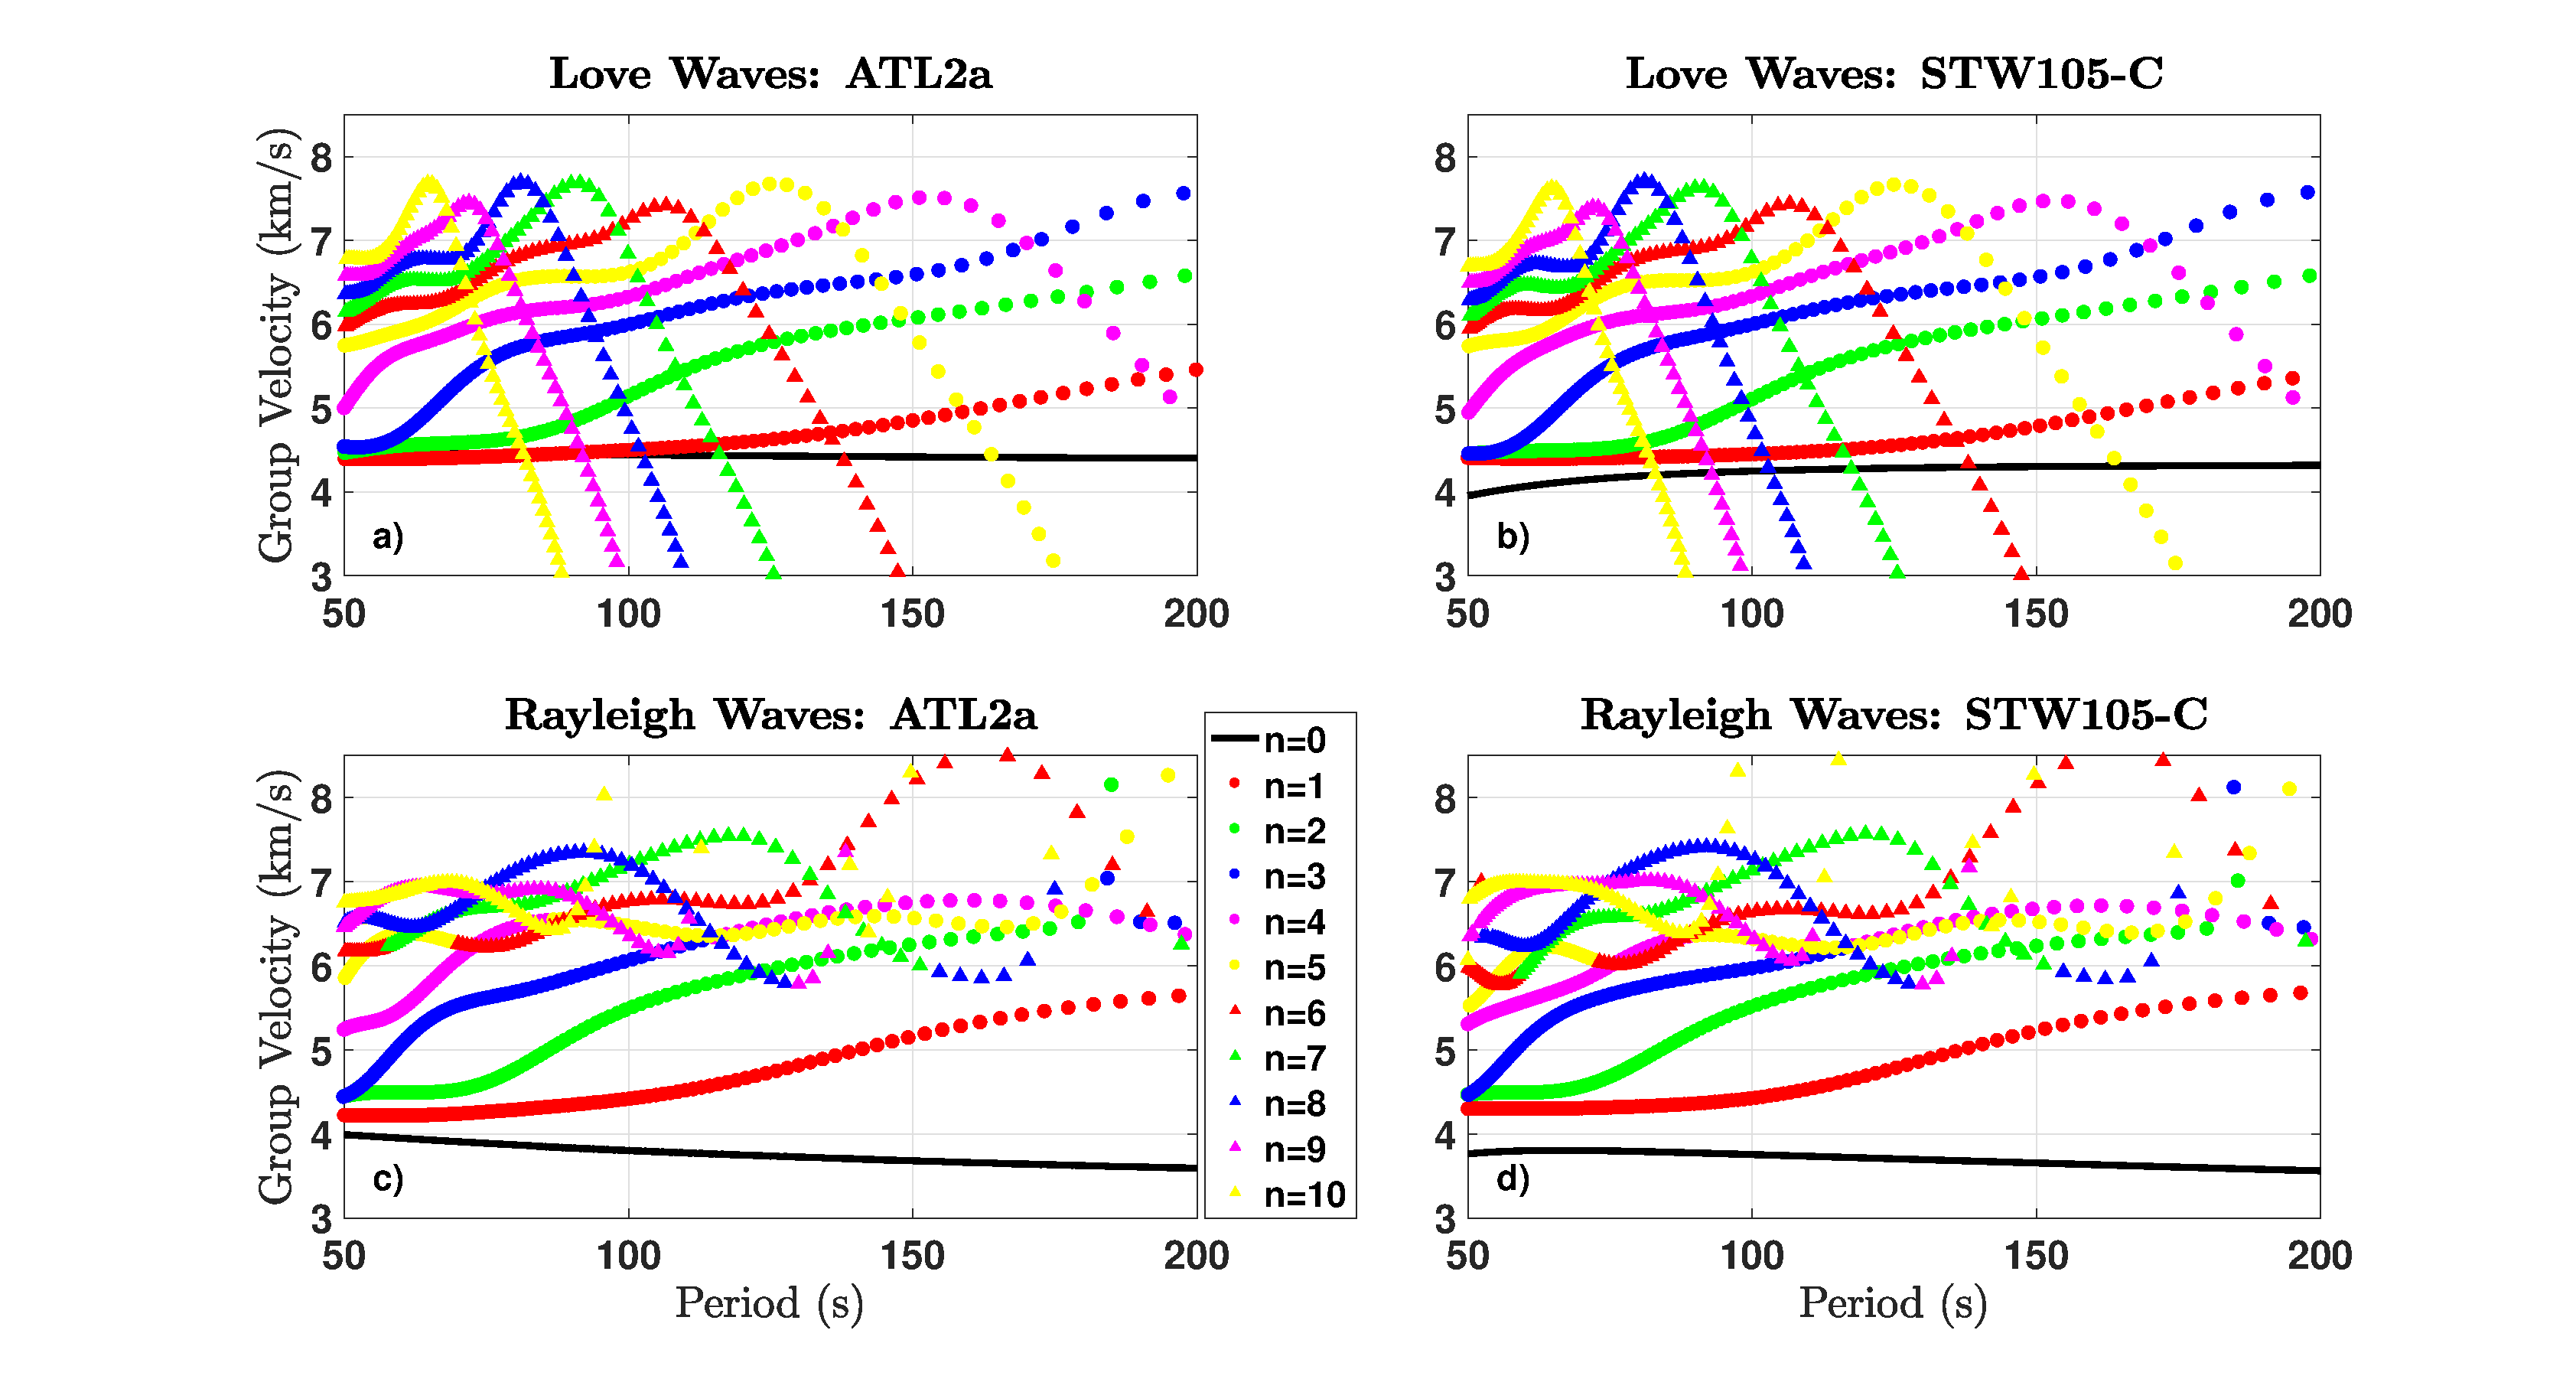
\includegraphics[width=1.0\textwidth]{Fig1_PostReviews.eps}
 \caption{Group velocities for the fundamental mode ($n=0$) and first ten overtones for (a) Love waves in an oceanic model, (b) Love waves in a continental model, (c) Rayleigh waves in an oceanic model, (d) Rayleigh waves in a continental model. Each color corresponds to a different radial order \textit{n}.}
 \end{figure}
 
 The fundamental requirement for overtone interference is that the group arrival times of the FM and the overtone overlap. Fig.\ 1 shows the group velocities of toroidal and spheroidal normal modes for radial orders $n=0-10$. The focus of this paper is propagating Love and Rayleigh waves, and in what follows we directly relate the overtone number or branch of the traveling wave to the radial order of the equivalent normal mode. Thus, the first overtone branch corresponds to n=1 and so forth. We show group velocities for both continental and oceanic settings, using the Earth model STW105-C, which is STW105 \citep{kustowski2008anisotropic} modified to have a 42-km-thick crust, for the continental setting and ATL2a \citep{james2014rayleigh} for the oceanic setting. 

At a given period, group velocities generally increase with  overtone number $n$, although this relationship is not apparent for Rayleigh waves with $n > 4$.  Rayleigh wave overtone group velocities that exceed the vertical scale correspond to Stoneley modes, which have sensitivity near the core-mantle boundary and are not well excited by the sources discussed in this study. Similarly, the high-$n$ Love wave group velocities that decrease abruptly at longer periods correspond to the core-reflected $ScS_{SH}$ phase \citep{dahlen1998theoretical}, and their overlap with the FM does not represent a significant contribution to overtone interference due to the low excitation of these modes.

Fig.\ 1 shows that the requirement of group arrival time overlap between an overtone and the FM is fulfilled for Love waves at periods less than 120 s, for which the group velocities of the FM and the first overtone are nearly the same. For continental settings, the Love wave group velocities of the first overtone and FM are close at intermediate periods but are well separated at periods less than 60 s \citep{nettles2011effect}. For the oceanic model, the first, second and perhaps even third Love wave overtones overlap with the FM at the shortest periods. On the other hand, for Rayleigh waves the group arrival times of the minor-arc overtones and minor-arc FM are consistently well separated due to large differences in the group velocities of the overtone and FM branches, except at the shortest periods for oceanic paths.

The large difference in Rayleigh wave group velocities between the FM and overtones causes the major-arc overtones to intersect the FM at intermediate to large epicentral distances, thereby contaminating FM measurements at those distances. The epicentral distance at which this intersection takes place can be estimated using Equation 1,  which we arrived at by equating the group arrival times of the fundamental-mode and major-arc overtone, where $U_{0}$ and $U_{1}$ are the group velocities of the FM and overtone of interest at a specific period, in km/s, $R_e$ is the radius of the Earth in km, and $X_{intersect}$ is the epicentral distance (in km) at which the overtone and FM intersect.

\begin{equation}
X_{intersect} = \frac{2 \pi R_e U_{0}}{U_1 + U_{0}}
\end{equation}
     
Fig. 2 plots $X_{intersect}$, calculated using the oceanic group velocities, as a function of period and overtone number. At shorter periods, the intersection distances tend to be slightly larger as a result of the generally slower overtone group velocities, whereas at longer periods the intersection distances are mostly concentrated between 115-160$^\circ$. 
       
\begin{figure}
\centering
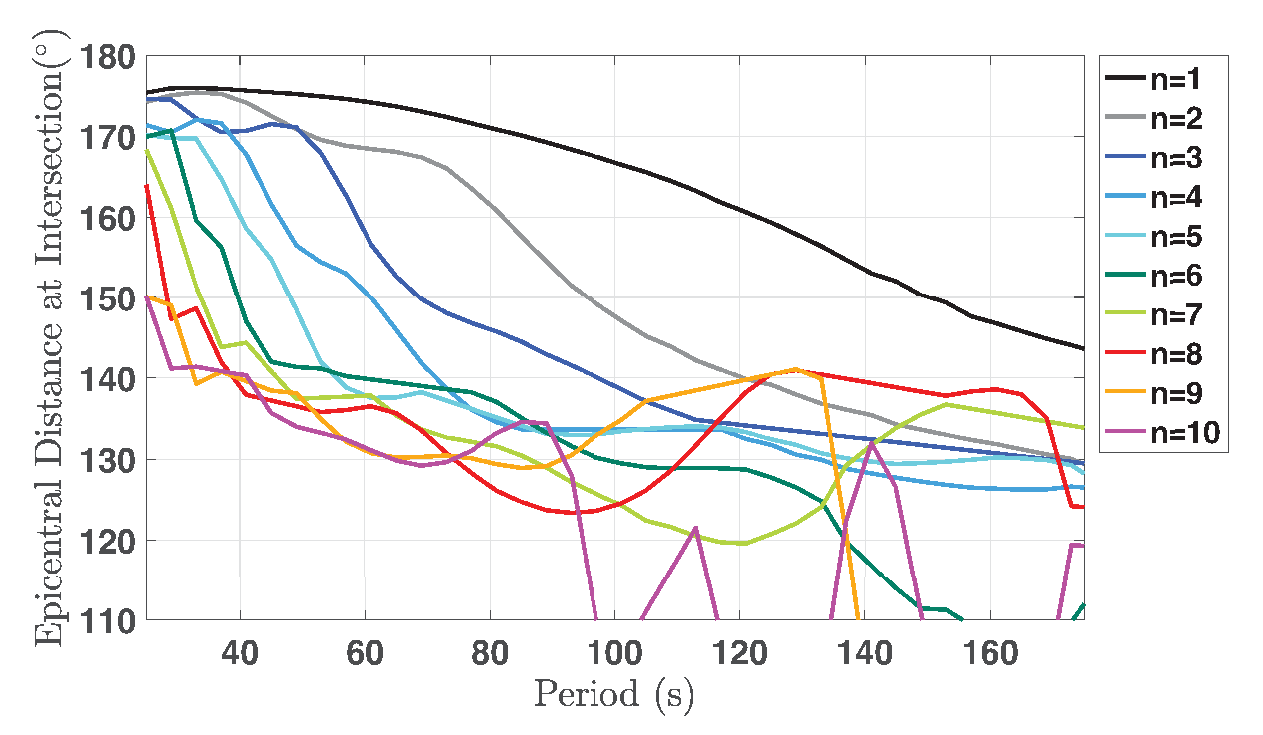
\includegraphics[width=0.95\textwidth]{Fig2_Sver.eps}
\caption{Epicentral distance at which the Rayleigh wave minor-arc FM and major-arc overtone intersect, calculated using Equation 1 for the oceanic model ATL2a. Each color corresponds to a different radial order \textit{n}. For ease of visualization, Stoneley modes are omitted in this figure. }
\end{figure}

When the FM and overtone group arrival times overlap, interference can occur. \citet{forsyth1975new} and \citet{thatcher1969higher} presented the following expressions for the effect of two-plane-wave interference on surface-wave phase $\phi$ (in radians) and amplitude $A$

\begin{subequations} 
\begin{align} 
\phi(\omega, x) = \tan^{-1} \left(\frac{\sin(\omega x/c_0) + \delta a \sin(\omega x/c_1) }{\cos(\omega x/c_0) + \delta a \cos(\omega x/c_1)} \right) \label{eqn: frobenius 7} \\ 
A(\omega, x,t) = (1 + \delta a^2 + 2 \delta a \cos[( \omega/c_0 - \omega/c_1)x])^{\frac{1}{2}} e^{-i ( \omega t)} \label{eqn: frobenius 8} 
\end{align} \end{subequations}


where $\delta a$ is the amplitude ratio of the overtone to FM, $c_0$ and $c_1$ are the FM and overtone phase velocities, respectively, $\omega$ is angular frequency,  $x$ is epicentral distance, and $t$ is time.
From Equation 2b it is clear that the wavenumber of the interference pattern multiplies $x$ inside the cosine term and thus the wavelength of the interference pattern can be rewritten as:
\begin{equation}
\lambda = \frac{T}{1/c_0-1/c_1},
\end{equation}

where $T$ is period. However, the apparent phase velocity of a major-arc overtone is negative, so  the expression for the wavelength of the interference pattern in the case of major-arc interference is:
\begin{equation}
\lambda_{major} = \frac{T}{1/c_0+1/c_1}. 
\end{equation}

The amplitude ratio $\delta a$ is critical to the strength of interference, and is governed by the relative source excitation of the FM and overtone surface waves. The Rayleigh wave source amplitude $R$ and Love wave source amplitude $L$ are given in equation 11.34 in \cite{dahlen1998theoretical}:
\begin{equation}
 \begin{aligned}
 R = |{} & \omega[(|M_{rr} \dot{U_s} + (M_{\theta \theta} + M_{\phi \phi}) r_s^{-1}(U_s-\frac{1}{2} kV_s)) e^{i \pi/4}  \\ & + (-1)^q (\dot{V_s} - r^{-1}_s V_s + k r^{-1}_s U_s)(M_{r \phi} \sin \Psi + M_{r \theta} \cos \Psi) e^{-i \pi/4}  \\ & - k r^{-1}_s V_s[M_{\theta \phi} \sin(2 \Psi) + \frac{1}{2}(M_{\theta \theta}-M_{\phi \phi}) \cos(2 \Psi)] e^{i \pi/4}]|
 \end{aligned}
\end{equation} 

\begin{equation}
\begin{aligned}
L = |{} & \omega((-1)^q (\dot{W_s} - r^{-1}_s W_s)(M_{r\theta} \sin(\Psi) - M_{r \phi} \cos(\Psi)) e^{-i \pi/4}  \\
& - k r^{-1}_s W_s [\frac{1}{2} (M_{\theta \theta} - M_{\phi\phi}) \sin (2 \Psi) - M_{\theta \phi} \cos (2 \Psi)]e^{i \pi/4})|
\end{aligned}
\end{equation}

where $\omega$ is the angular frequency, $k$ is the wavenumber,  $M_n$ represents the components of the moment tensor, $r_s$ is the source radius, $\Psi$ is the azimuth measured counterclockwise from south, $q$ is the wavegroup index, and $U_s$, $V_s$, $W_s$, $\dot{U_s}$, $\dot{V_s}$, and $\dot{W_s}$ are the normalized displacement eigenfunctions and their derivatives, respectively, evaluated at the source depth.

\section{Data and Measurements}
\subsection{Normal-Mode Synthetic Seismograms }
We rigorously explore the extent of overtone interference for a range of example source mechanisms and depths. We use synthetic seismograms calculated for a known 1-D Earth model via normal-mode summation \citep{gilbert1971excitation}. The mode eigenfunctions and eigenfrequencies are computed with the MINEOS code \citep{mineosbro}. The summation includes all modes with frequency $< 50$ mHz and angular order $< 500$. The advantage of mode summation is that it is computationally cheap and we can control which overtone branches (i.e., which values of $n$) are included in the seismograms.
For Love waves, the source excitation and group velocity (Fig. 1) of the FM and overtones differ substantially  for oceanic and continental models, and we repeat all calculations using ATL2a and STW105-C. For Rayleigh waves, the differences are minor, and we perform simulations using ATL2a only. 

We calculate synthetic seismograms for three example focal mechanisms and four source depths. We use focal mechanisms corresponding to a vertical strike-slip fault ($\delta=90^\circ$, $\lambda=0^\circ$), a dip-slip fault dipping at 45$^\circ$ ($\delta=45^\circ$, $\lambda=90^\circ$), and a dip-slip fault dipping at 90$^\circ$ ($\delta=90^\circ$, $\lambda=90^\circ$), where $\delta$ is the dip angle and $\lambda$ is the slip angle. We will refer to the latter as a vertical dip-slip fault. We use source depths of 12, 62, 112, and 162 km. When calculating the synthetic seismograms, stations are placed along a great-circle path at approximately 1$^\circ$ spacing. For consistency, the position of the stations changes for each event and is chosen so that the azimuth of the linear array corresponds to a maximum in the FM radiation pattern for the source of interest. Our choice to conduct these illustrative calculations along this azimuth corresponding to the largest FM radiation pattern is purely arbitrary, and only serves to illustrate the key point that observations of overtone interference are consistent with predictions of the strength of interference, based on excitation ratio calculations. While we do not explicitly show examples at other azimuths, our calculations on real data, which take into account the azimuth from source to station, show agreement between predictions and results. We have conducted tests at other azimuths and find that excitation ratios as invariant as a function of azimuth for Love waves, and slightly variant as a function of azimuth for Rayleigh waves, though the trends we show here as a function of period and source depth behave similarly. 

We quantify the impact of overtone interference on the measurements of FM travel time and amplitude following the approach of \citet{hariharan2020evidence} and \citet{foster2014overtone}. We generate two sets of synthetic seismograms for every station: one includes the FM and overtones, and the other includes only the FM. FM travel time and amplitude are measured for both sets (Section 2.2). The measurements made on synthetic seismograms that contain overtones and the FM are  expressed relative to their values measured from the synthetics containing only
the FM; the travel times are differenced and the amplitudes are divided. In doing so the effects of the source radiation pattern, attenuation, and geometrical
spreading will be cancelled out, allowing the effects of higher-mode interference to be isolated. We refer to these representations of the measurements as ``the travel-time interference pattern'' and ``the amplitude interference pattern''. Deviations of the travel-time interference pattern from zero and of the amplitude interference pattern from one are evidence of overtone interference effects.

\subsection{Measurement Methods and Phase Velocity Calculations}

To make measurements of the travel time and amplitude of the Rayleigh and Love waves in the normal-mode synthetic seismograms, we use Fourier analysis \citep{forsyth2005array}. With this approach, a window is defined based on the expected surface-wave arrival. The window is centered on the predicted group arrival time (Fig.\ 1), and its length is equal to twice the period of the wave. A Tukey taper (tapered cosine) is applied to the center half of the window. We have experimented with larger window lengths and find that both the amplitude and travel-time measurements and the resulting interference patterns depend negligibly on the window length apart from a very minor increase in interference as window length increases for Rayleigh waves. After windowing, the seismograms are bandpass filtered with a filter width equal to one-tenth of the center period. After taking the Fourier transform of the windowed and filtered seismogram, we extract the phase from the angle corresponding to the ratio of the real and imaginary components. The phase is unwrapped after sorting with increasing epicentral distance so that it increases with distance instead of being restricted to the range of the arctangent function. The modulus of the real and imaginary components is used to estimate amplitude. 

We have found that this Fourier approach is more stable for our measurements on normal-mode synthetics than the Automated Surface Wave Measuring System \citep{jingmcc}, which we have successfully applied to real data from the EarthScope USArray (Section 2.3). The reason is that, in trying to comprehensively characterize overtone interference, our study includes some synthetic seismograms that have very weak FM excitation and are dominated by overtones. We have found that ASWMS works very well for seismograms with a prominent FM, which is what it was developed for, but is prone to instability when the FM is weak. Fig.\ S1 shows that ASWMS and the Fourier approach produce similar travel-time measurements for seismograms with weak overtone interference but differ when overtone interference is very strong.  

We quantify how overtone interference impacts phase velocity using Eikonal tomography \citep{lin2009eikonal}, which applies the Eikonal equation (Equation 7) to the measured travel-time field $\tau$,  
\begin{equation}
\frac{1}{c^2} = \nabla \tau \cdot \nabla \tau
\end{equation}
\noindent
where $c$ is 2-D phase velocity. In practice, the travel-time measurements are first averaged in 0.5$^\circ$ cells, then interpolated onto a smooth surface. We use the algorithm of \citet{smith1990gridding} implemented in GMT \citep{wessel1998new}, which solves for a minimum-curvature surface under tension. We interpolate onto a grid of $0.25^\circ \times 0.25^\circ$ cells. The gradient term is calculated using a finite-difference method in spherical coordinates. This process is
performed separately for each event, and the event-specific Eikonal phase-velocity maps are determined from the reciprocal of $\sqrt{|\nabla \tau|^2}$. 

\subsection{Real Data: USArray Measurements}

In Section 4, we explore the impact of interference on real Rayleigh and Love wave measurements made at EarthScope USArray stations. 
For Rayleigh waves we use the data set of \citet{babikoff2019long} for earthquakes that occurred during 2007-2014. These measurements were made using the Automated Surface-Wave Measuring System (ASWMS) \citep{jingmcc}, which utilizes multi-channel cross-correlation of waveforms at nearby stations. For each event, single-station travel times are obtained from the inter-station delay times using a least squares approach, and the single-station amplitudes are determined from the square root of the peak of the auto-correlation function of the windowed Rayleigh wave. For Love waves we use a data set measured with the approach of \citet{ekstrom1997measurements}, which utilizes a phase-matched filter to determine single-station travel times and amplitudes relative to a synthetic seismogram. The Love wave data set contains earthquakes that occurred between 2006 and 2015. Our results should not be affected by the fact that we use Rayleigh and Love wave data sets measured with different approaches.  \citet{hariharan2020evidence} showed that the Rayleigh wave major-arc overtone interference is not unique to a particular measurement technique; it is present in data sets measured with ASWMS and the approaches of \citet{ekstrom1997measurements} and \citet{ma2014comprehensive}. \citet{jingmcc} showed that the Love wave overtone interference is also detectable using ASWMS, and \citet{foster2014overtone} showed that it was detectable using the technique of \citet{ekstrom1997measurements}.

\section{Results of Tests with Synthetic Seismograms}

In this section, we use measurements on normal-mode synthetic seismograms to characterize patterns in the strength of overtone interference for Rayleigh and Love waves. We examine to what extent these patterns can be explained by the relative excitation of the FM and overtones. 
\subsection{Love Wave Interference}
 
For Love waves, the relative excitation of the FM and first overtone is often considered to exert first-order control on interference strength, as a result of the closeness of the group-velocity curves. Fig.\ 1a shows that at short periods the second and even third overtone may also influence interference for an oceanic velocity model; this is explored later in this section. Using Equation 6, we  calculate excitation as a function of source depth for the FM and first overtone for the three example source mechanisms described in Section 2.1; Fig.\ S2 shows the raw excitation as a function of depth, and at different periods. Fig.\ 3 shows the ratio of the excitation of the first overtone and FM, where larger values correspond to larger relative excitation of the first overtone. Whenever excitation ratio is referred to or shown in this paper, the excitation of the FM is in the denominator.
\begin{figure}
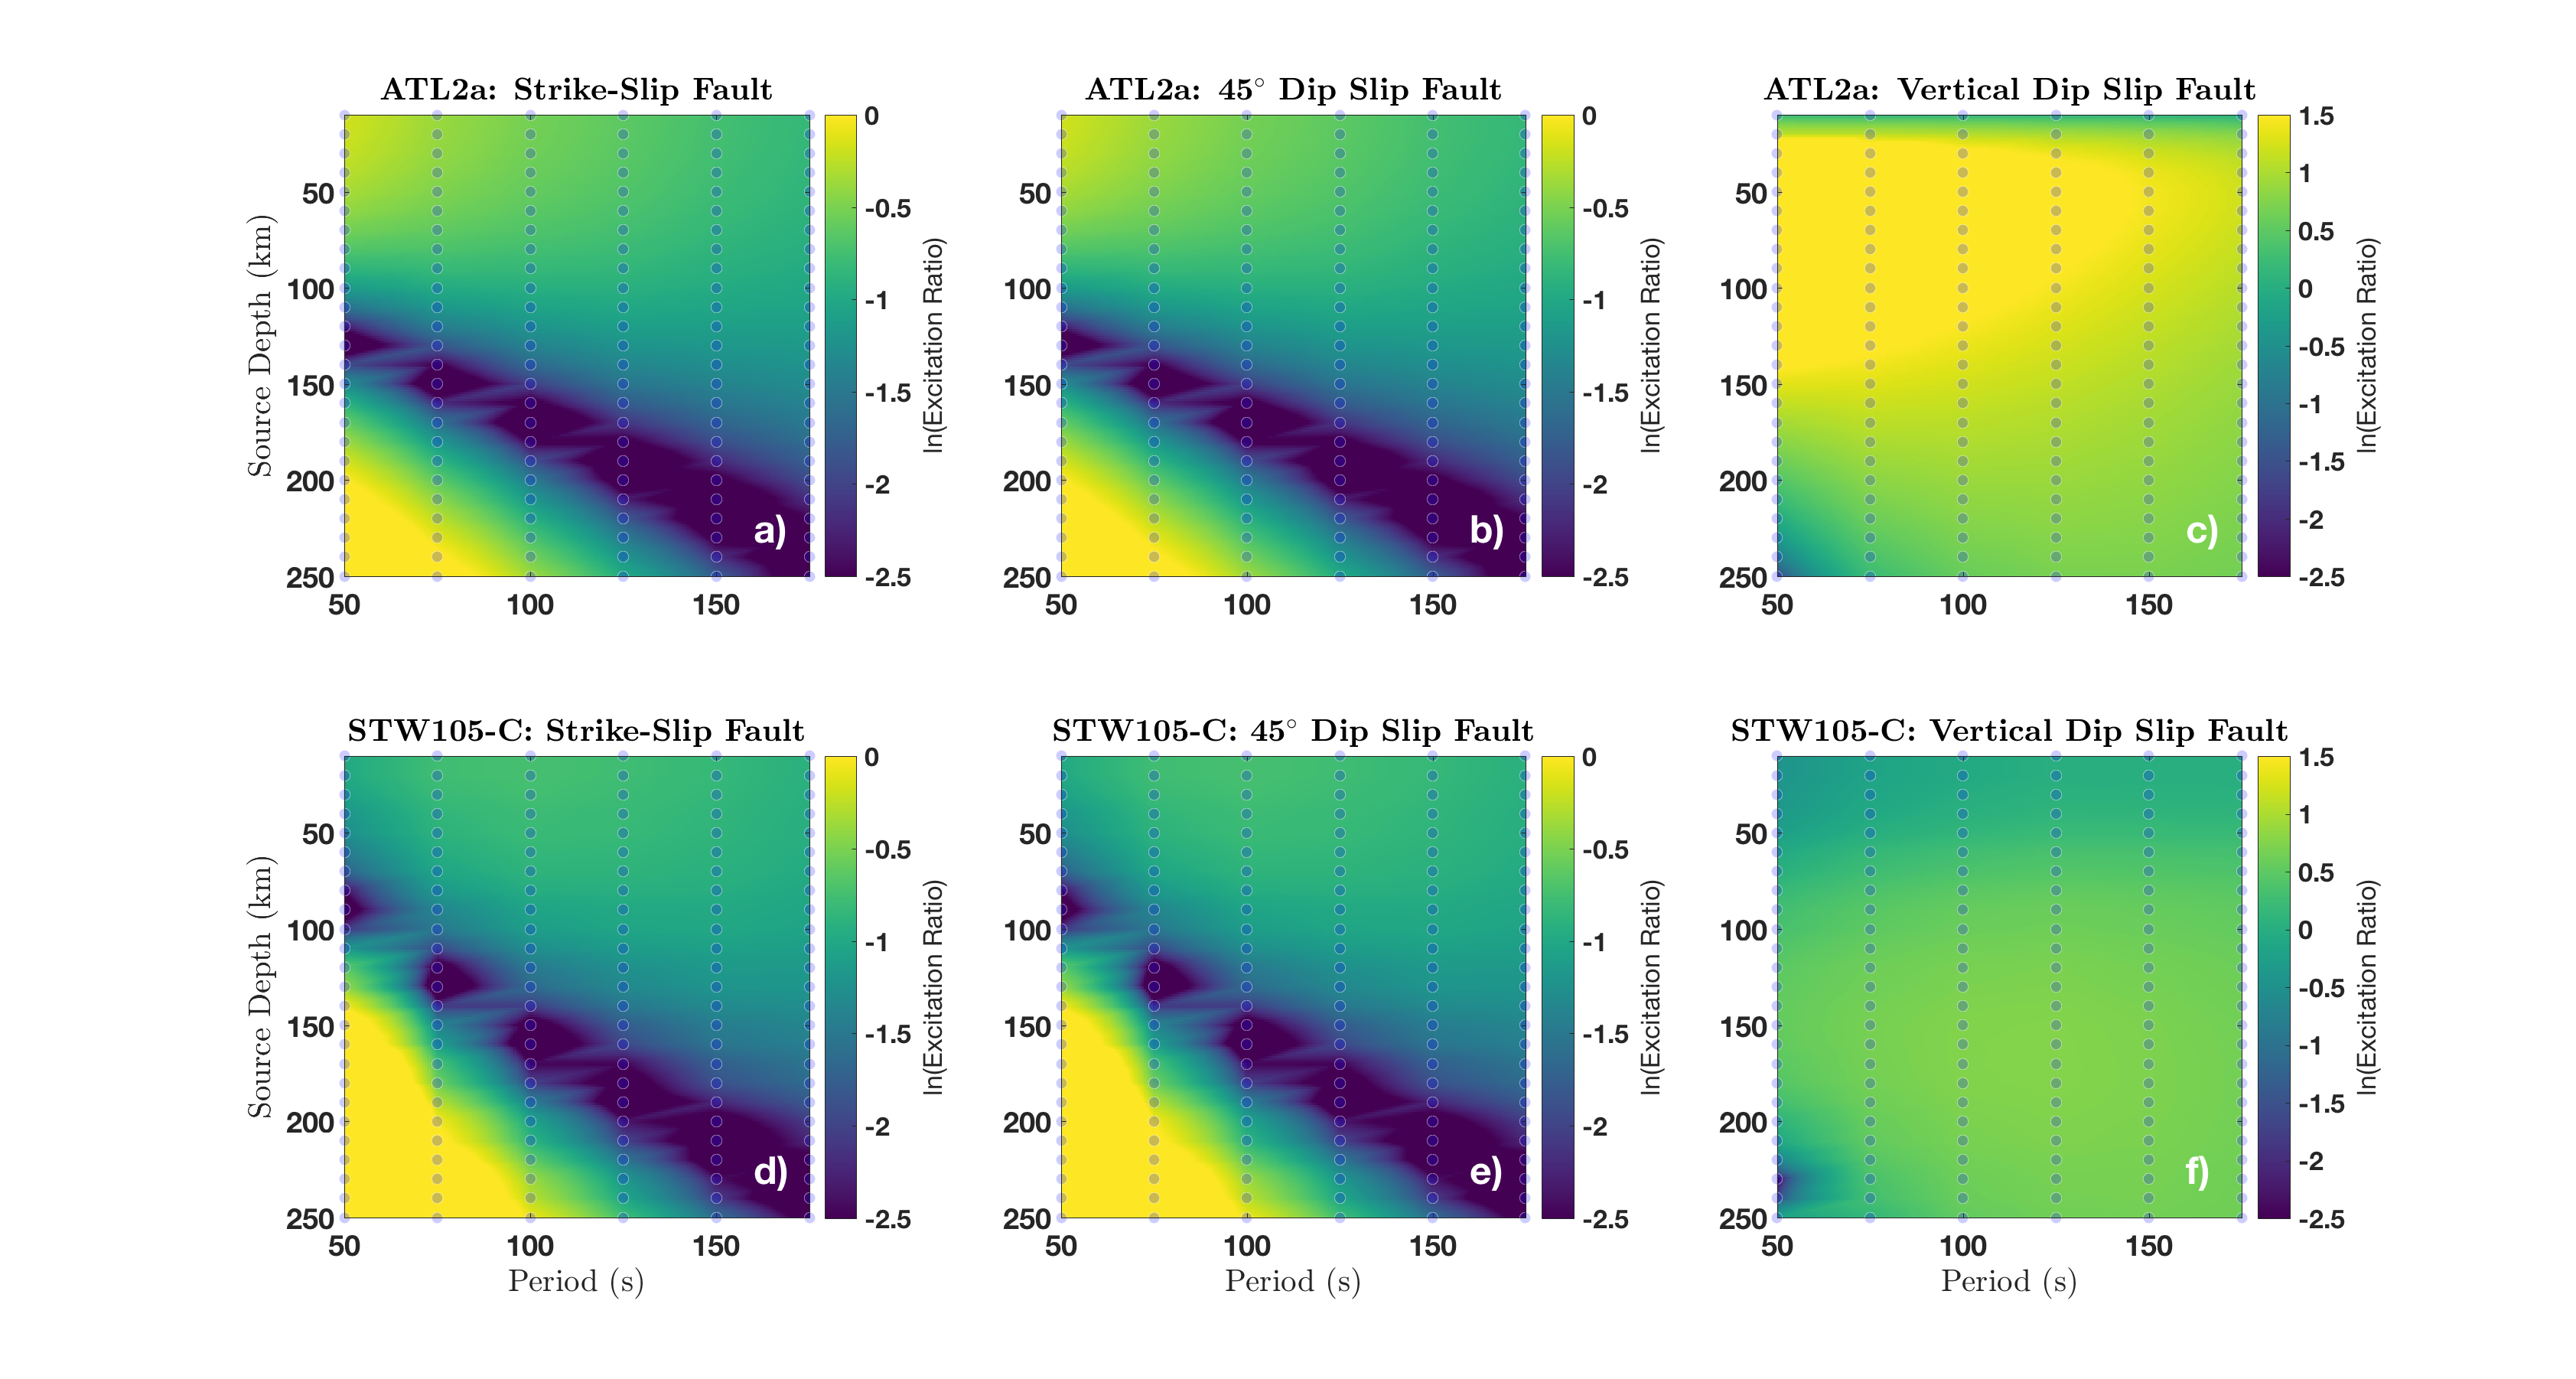
\includegraphics[width=1\textwidth]{Fig3_CorrectedColorbar.eps}
\caption{Ratio of Love wave excitation: first overtone excitation with respect to the FM excitation. (a-c): Calculations for ATL2a. (d-f): Calculations for STW105-C. Each column is a different example source. The points at which this function is evaluated are plotted as blue dots; these excitation ratios have been interpolated to form the color surface. Note the different range of excitation ratios on the third column as compared to the first and second.}
\end{figure}
The excitation ratios for strike-slip and 45-degree dip-slip faults are identical, although the magnitudes of the 45-degree dip-slip excitation are larger. For both of these faults, the excitation of the first overtone exhibits a minimum in excitation at a depth that increases with increasing period, from approximately 125 km at 50 s to around 250 km at 175 s. This minimum also broadens in depth with increasing period. As a result, the excitation ratios for these fault types also contain minima, the depths of which vary systemically with period (Fig. 3). For the vertical dip-slip fault, the excitation of the first overtone is almost always larger than the excitation of the FM, resulting in excitation ratios $>$ 1. 

\begin{figure}
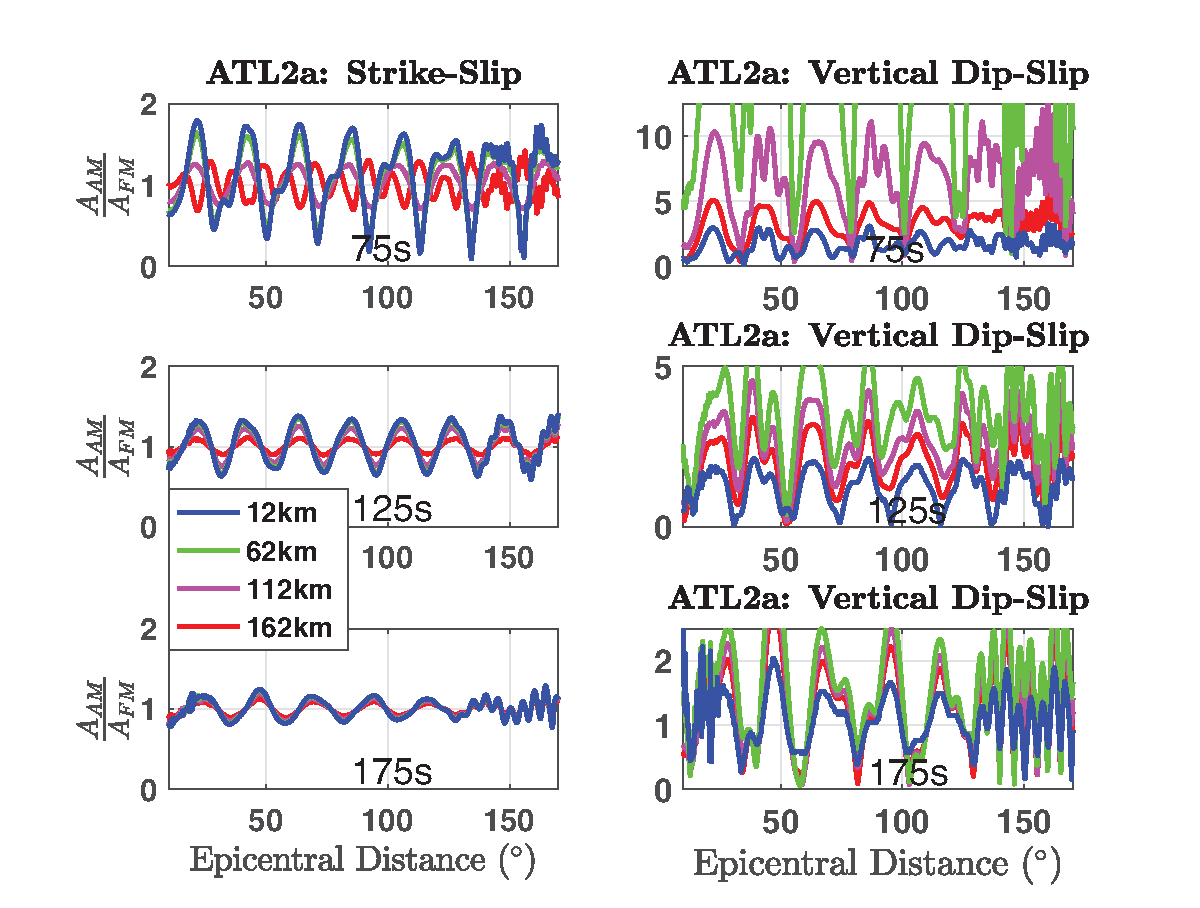
\includegraphics[width=1\textwidth]{Fig4_LargerYAxes.eps}
\caption{Amplitude interference patterns for Love waves, showing the ratio of amplitudes measured from synthetic seismograms containing all modes to those measured from synthetic seismograms containing only the FM. Simulations are for example events and four source depths. Note the different y-axis ranges for panels in the right column.}
\end{figure}
 
We have found that variations in the character of overtone interference as a function of source depth, as inferred from normal-mode synthetic seismograms, are well explained by variations in the Love wave excitation ratios. As described in Section 2.1, we computed synthetic seismograms for the three example events at four depths. Fig.\ 4 shows the amplitude interference patterns that we determined from them. We do not show results for the 45-degree dip-slip event since they are identical to the strike-slip event. Examples of travel-time interference patterns can be found in Fig. S4.. At a given period in Fig.\ 4, all four curves (source depths) have the same group velocity; differences between them are thus due to source excitation. For the strike-slip fault at 75 s, Fig.\ 3a suggests that overtone interference should be largest for source depths approximately $<$ 75 km and $>$ 175 km, and this is confirmed by amplitude interference patterns: the effect of Love wave overtone interference on amplitude is roughly twice as large for source depths of 12 km and 62 km than for 112 km and 162 km. Fig.\ 3a also hints that at 125 s the relative excitation of the first overtone is weak for a strike-slip fault at 162 km, which is corroborated by the small interference effects in Fig.\ 4b. On the other hand, Fig.\ 4d-f show clearly that overtone interference is very strong for the vertical dip-slip fault, as expected from Fig.\ 3c. In particular, measurements at short periods and shallow depths in Fig.\ 4d show the strongest overtone interference for the vertical dip-slip fault, reflecting correspondingly large excitation ratios at short periods and shallow depths. Fig.\ 4f shows that at 175 s for vertical dip-slip faults, interference effects are smallest for a source at 12 km, which is consistent with the depth dependence of excitation ratios in Fig.\ 3c. 

 \begin{figure}
 \includegraphics[width=1.0\textwidth]{Fig5_Sver.eps}
 \caption{Love wave amplitude interference patterns, color-coded by period (s), for the FM and first overtone (a,d), second overtone (b,e), and third overtone (c,f). The absolute difference (in km/s) between the group velocities of the FM and overtone is indicated in parentheses next to the period label. In all cases the source mechanism and depth are chosen such that the ratio of overtone to FM excitation is approximately unity. Thus, differences between the interference patterns in the left-hand and right-hand columns are due entirely to the different group velocities of the oceanic and continental Earth models. }
 \end{figure}
 
The Love wave interference patterns are affected by the proximity of FM and overtone group velocities in addition to the relative excitation of the FM and overtones. We explore the role of group-velocity proximity in Fig.\ 5, where we isolate the interference effects from the first, second, and third overtones, since group-velocity separation generally increases with overtone number (Fig. 1a,b). In each case we choose a source mechanism and depth so that the overtone-to-FM excitation ratio is approximately unity. Fig. 5 makes clear that group-velocity proximity controls both the strength and distance-dependence of interference. If the group velocities are close (within $ \sim 0.25$ km/s), interference strength is constant across the distance range with a magnitude that scales with degree of velocity closeness (Fig. 5a). If the group velocities are better separated, the interference strength depends strongly on distance as the overtone wave packet moves ahead of the FM wave packet. This is illustrated by the interference between the FM and second overtone in Fig. 5b. At the longest periods, interference decays with distance as a consequence of the well separated group velocities. The shortest periods, where group velocities overlap, show stronger interference that varies little with distance. The role of group-velocity separation is especially evident in the comparison of interference patterns computed for the oceanic (Figs. 5a-c) and continental (Figs. 5d-f) velocity models. The short-period group velocities in the continental model are lower and therefore better separated from the overtones than in the oceanic model. As a result, 50-s interference is very weak for STW105-C.

Group-velocity separation has two additional consequences for the Love wave interference patterns in Fig. 4. Firstly, a secondary oscillation in amplitude ratio is superimposed on the dominant signal that is due to interference from the first overtone, (this secondary oscillation is visible in Fig.\ 4a, appearing more clearly as a distinct interference pattern for the source at 162 km or as a local maximum in between the more dominant peaks and troughs for the source at 12 km) which reflects the fact that both the first and second overtones are able to interfere with the FM at short periods. Secondly, the short-wavelength signal that modulates the interference pattern at distances $> 130^\circ$  reflects interference from Love wave overtones traveling along the major arc.

The velocity model has a second-order effect on the overtone-to-FM excitation ratio (Fig. 3) and therefore a second-order effect on the interference pattern. For example, for the vertical dip-slip fault, the relative excitation of the first overtone is smaller for STW105-C than for ATL2a. As a result, interference is slightly weaker for STW105-C than ATL2a, which can be seen by comparing Figs. 4f and S3l.

 
In Fig. 6, the effects of velocity model, source depth and mechanism, and period on Love wave interference are summarized using a single quantity, which is the maximum value of the amplitude interference pattern for epicentral distances between 30$^\circ$ and 90$^\circ$. It illustrates the larger interference for vertical dip-slip faults than strike-slip faults and for the oceanic model than the continental model. The effect of source depth depends on the fault type. For strike-slip faults, the shallowest events produce stronger Love wave overtone interference, whereas for vertical dip-slip faults the deeper events have stronger interference
 
  \begin{figure}
 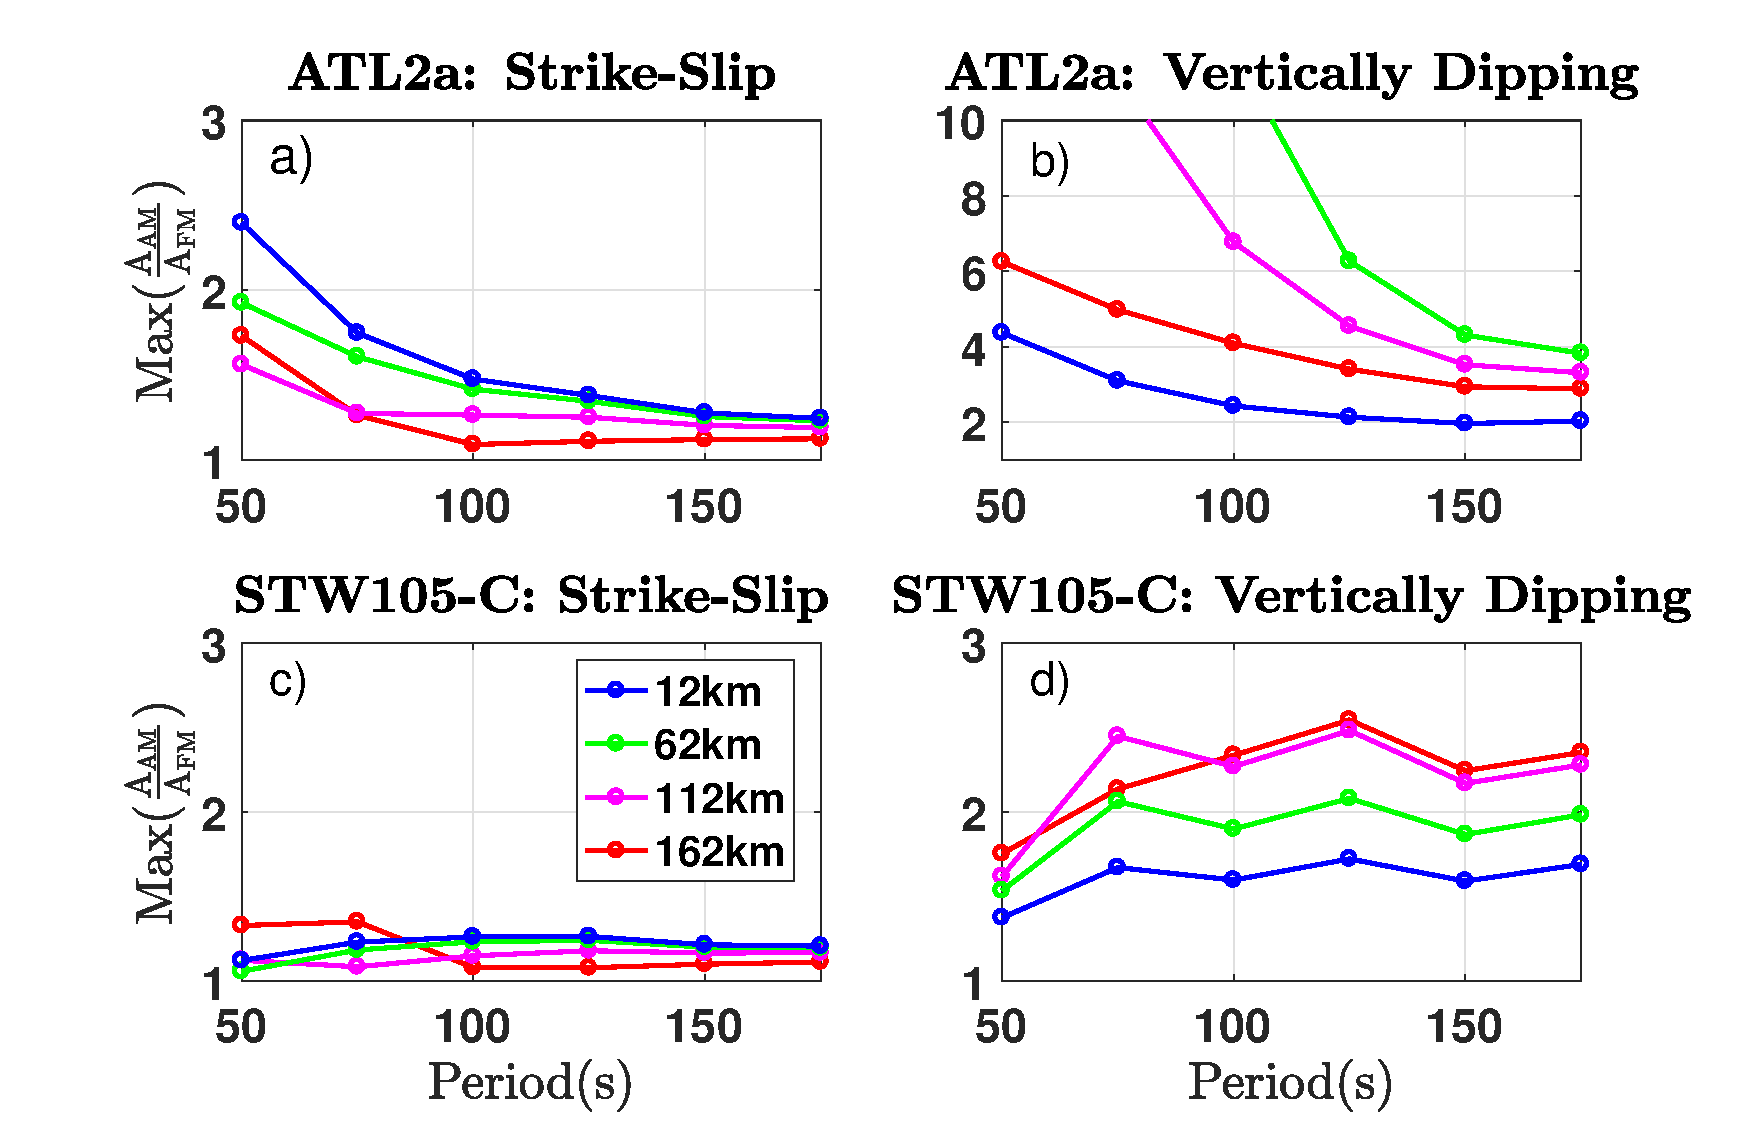
\includegraphics[width=1.0\textwidth]{Fig6_Sver.eps}
 \caption{Summary of the strength of Love wave amplitude interference as a function of period, velocity model, and source mechanism and depth. Note the different y-axis range on panel b). }
 \end{figure}

\subsection{Rayleigh Wave Interference}

 For Rayleigh waves, we must consider many overtone branches, since the interference is not controlled by closeness of group velocities as it is for Love waves, and multiple overtones can intersect the FM at certain distances (Fig.\ 2). Fig.\ 7 shows the excitation as a function of depth for the example fault types (Equation 5), calculated for the FM Rayleigh wave and first ten overtones. An important feature of these excitation functions is the minimum in FM excitation for the strike-slip and 45-degree dip-slip faults. The depth of the minimum increases with increasing period. For strike-slip faults, the depth of the FM excitation minimum increases from approximately 50 km to 110 km between 50 s and 175 s. For 45-degree dip-slip faults, it increases from approximately 25 km at 50 s to 100 km at 175 s. For vertical dip-slip faults, the FM is more excited than the overtones, except for large depths at short periods. The  overtone excitations also contain minima at certain depths, which means that source depth will influence which overtones interfere with the FM at a given period.  
 
      \begin{figure}
 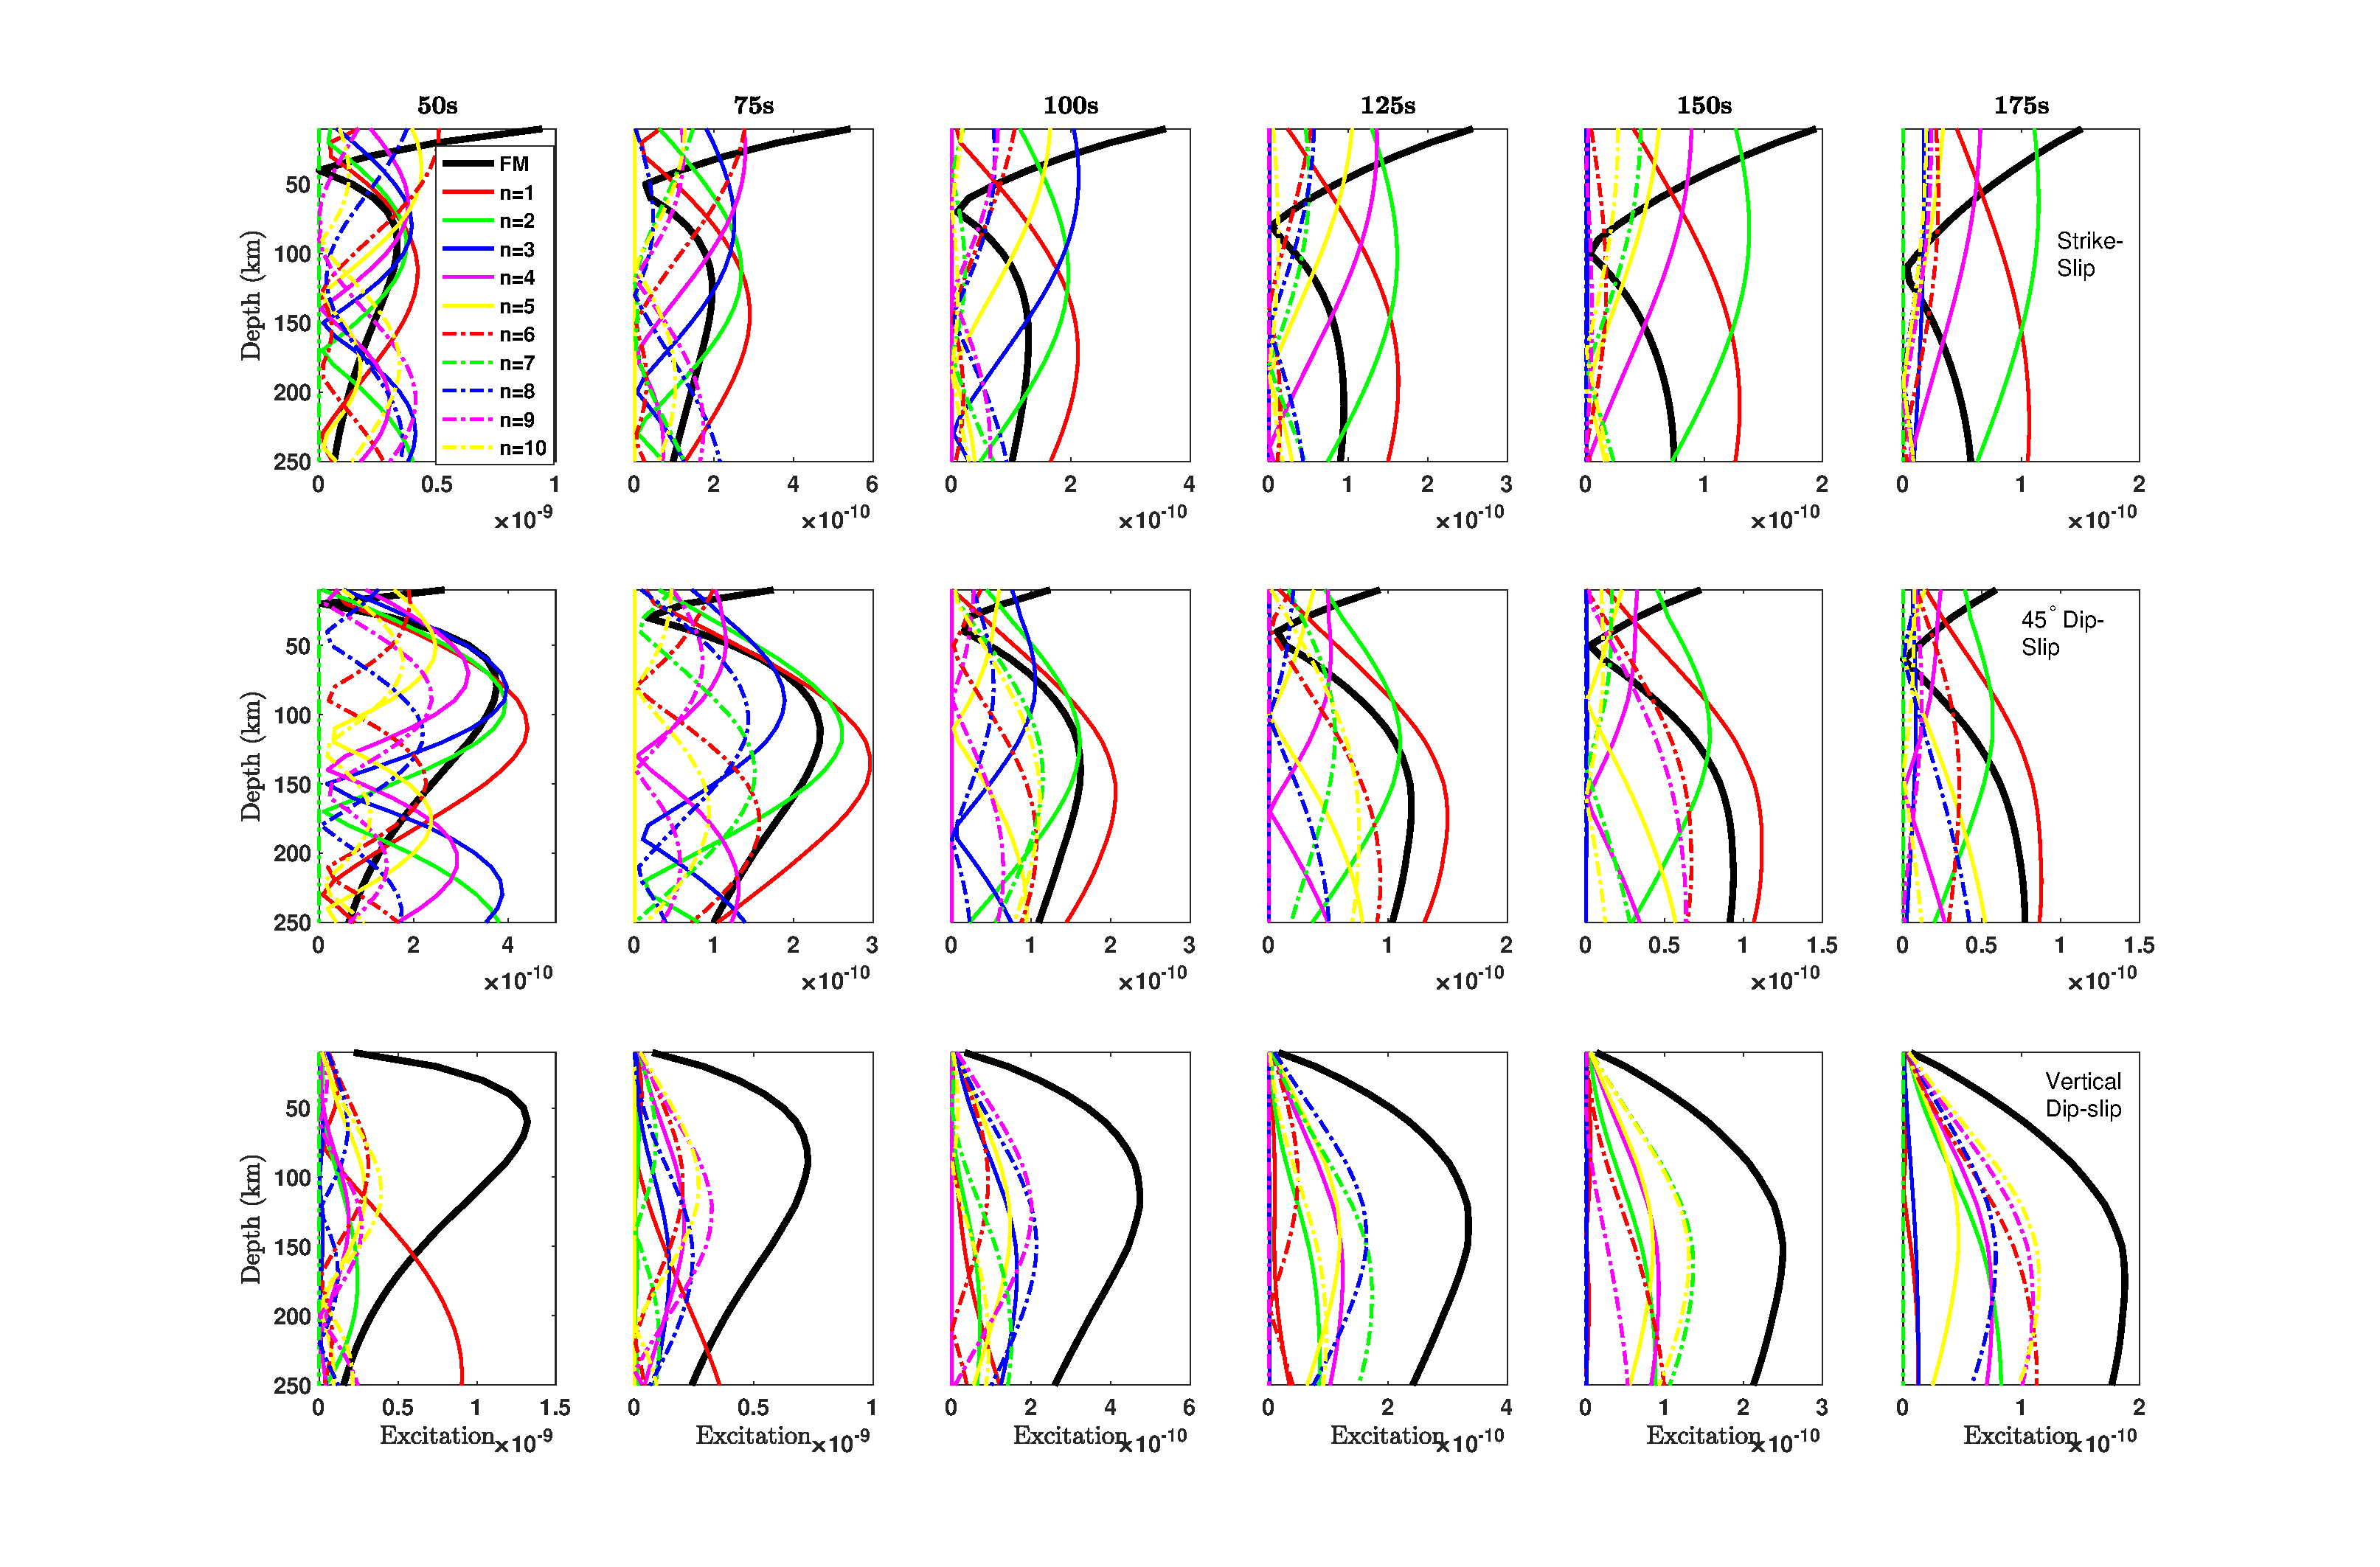
\includegraphics[width=1.0\textwidth]{Fig7_CorrectedColor.eps}
 \caption{Rayleigh wave excitation for the fundamental mode and first ten overtones as a function of depth for the three example source mechanisms. Calculated for the oceanic velocity model.}
 \end{figure}

 Figs.\ 8 and 9 show that relative excitation of Rayleigh wave overtones and FM exerts strong control on the interference effects in amplitude measurements as determined from normal-mode synthetic seismograms. Fig.\ 8 focuses on the distance range where major-arc overtone interference dominates, and Fig.\ 9 focuses on the distance range where minor-arc interference dominates. Unlike the Love wave amplitude interference patterns in Fig.\ 4, we show only the top half ($\frac{A_{AM}}{A_{FM}}>1$). It is clear from Fig.\ 8 that the strength of major-arc overtone interference varies dramatically as a function of epicentral distance, source depth, and fault type. To evaluate the role of overtone excitation in controlling both the strength and distance dependence of interference, we plot as circles the excitation ratios for the first ten overtones at the distance where they intersect the FM; a large excitation ratio corresponds to large relative excitation of the overtone.

\begin{figure}
 \includegraphics[width=0.99\textwidth]{Fig8_Sver.eps}
 \caption{ Left vertical axis shows Rayleigh wave amplitude interference pattern (top half only) in the distance range prone to major-arc interference. Right vertical axis shows Rayleigh wave excitation ratios (overtone excitation / FM excitation) for the first ten overtones, plotted as circles at the distances at which the overtones intersect the FM and colored by source depth. }
\end{figure}
     
         \begin{figure}
 \includegraphics[width=0.99\textwidth]{Fig9_Sver.eps}
 \caption{As in Fig.\ 8 but in the distance range prone to minor-arc interference. The Rayleigh wave amplitude interference patterns (top half only) are plotted with solid lines. The excitation ratio of the first overtone relative to the FM is plotted as a horizontal dashed line across the entire distance range. }
     \end{figure}     
     
 For a given source mechanism and period, Fig.\ 8 shows that source depth is the dominant control on the strength of major-arc overtone interference. The excitation ratios, shown as circles, also depend strongly on source depth, and the source depths that produce the strongest Rayleigh wave interference also have the largest excitation ratios (e.g., 62 km at 100s for Strike-Slip and $45^\circ$ Dip-Slip faults, and 112 km at 150s for a Strike-Slip Fault). Thus, excitation ratio explains the overall strength of interference in the distance range prone to major-arc interference. Furthermore, the excitation ratios explain the modulation of the interference pattern as a function of distance. For instance, at 100 s for the strike-slip fault, interference is low between 100 and $120^\circ$ for all source depths, and the excitation ratios for the overtones that intersect the FM in this distance range are very small. On the other hand, the excitation ratios of the overtones that intersect the FM at distances $> 120^\circ$ are much larger, especially for the 62-km source, and peak at approximately $140^\circ$, consistent with the peak in the amplitude interference pattern determined from synthetic seismograms. 

The source depth that produces the largest interference varies with period and source mechanism, and comparison with Fig.\ 7 indicates that the relative excitation of the FM is the dominant factor controlling this variation. At 150 s, it is the 112-km event for the strike-slip fault and the 62-km event for the 45-degree dip-slip fault. These depths are close to the minima in FM excitation for these two fault types, thereby allowing a larger contribution for overtones. Another factor that influences the shape of the interference pattern is whether any overtones intersect the FM. Many of the interference patterns show little interference in the distance range $155-165^\circ$, which can be attributed to an absence of overtone intersections in this distance range.  
 
Vertical dip-slip faults generally have very low excitation ratios as the FM is generally the most strongly excited at depths $<$ 250 km. Consequently, the amplitude interference pattern is small. In summary, our analysis shows that the overtone excitation ratios, when considered in context with the distance at which each overtone intersects the FM, can explain the characteristics of the major-arc interference pattern, including its distance dependence and strength. 

At shorter epicentral distances, we find that  interference of minor-arc Rayleigh wave overtones, especially the first overtone, with the FM can be strong under certain circumstances. Fig.\ 9 plots the minor-arc interference pattern in amplitudes overlain with the excitation ratio of the first overtone and FM as a horizontal line corresponding to the right-hand vertical axis. As in Fig.\ 8, the vertical dip-slip faults produce minimal overtone interference with the exception of the deepest source at short periods, where the first overtone has notable excitation (Fig.\ 7). The event at 12 km well excites the FM and weakly excites the first overtone for all periods and fault types, resulting in low interference for this source depth. Deeper events are characterized by excitation ratios $>$ 1 for the strike-slip and 45$^\circ$-dip-slip faults, and therefore the Rayleigh wave measurements exhibit substantial minor-arc interference. These excitation ratios control the strength of the interference pattern. For instance, at 150 s for the strike-slip fault, the excitation ratios sorted from largest to smallest are generated by sources at 112 km, 162 km, 62 km, and finally 12 km. The strength of the amplitude interference pattern determined from the synthetic seismograms follows the same order. 

As we found for major-arc overtone interference, the presence of a minimum in FM excitation exerts strong control on the excitation ratio of the first overtone with respect to the FM. At 100 s, for the strike-slip and 45-degree dip-slip faults, the FM excitation minimum occurs close to 62 km, resulting in the large minor-arc interference for this source depth. Fig.\ 9 shows that the separation of FM and first overtone group velocities introduces a decay in minor-arc interference with epicentral distance as the overtone moves out of the time window used in measurements. This decay rate is smaller at shorter periods, due to the relative closeness of the FM and first overtone group velocities.

Figs.\ 8 and 9 highlight the sharp contrast in the wavelength of major- and minor-arc overtone interference, with a much larger wavelength for the latter. Using synthetic seismograms for an explosive source and including only the first overtone and the FM to ensure the simplest possible interference pattern, we show in Fig.\ S5 that Equations 3 and 4 accurately predict the wavelength of the major and minor-arc interference that we measure from the amplitude interference patterns. Wavelength is measured by windowing the interference pattern in the relevant distance range, taking the Fourier transform of the interference pattern, and finding the wavelength that corresponds to the spectral peak. 

Figs.\ S6 and S7 show the complete Rayleigh wave amplitude and travel-time interference patterns, respectively, for several periods and the full range of epicentral distance. When the excitation ratio is very large (e.g., 100 s for the 62-km source depth and the 45-degree dip-slip fault), the travel-time interference pattern can take on a very different character, with unreasonably large time shifts and the absence of an oscillatory pattern, which we speculate occurs because the windowed seismogram is dominated by the overtone rather than the FM.

\subsection{Interference in a Realistic Event Distribution}

Having probed example source mechanisms, we now explore how well the tests in Sections 3.1 and 3.2 capture the diversity of interference in typical surface-wave data sets. We compute normal-mode synthetic seismograms and calculate the interference patterns, for both Rayleigh and Love waves, for 200 events in the Global CMT catalogue \citep{dziewonski1981determination,ekstrom2012global}. These 200 events are randomly selected from the subset that occurred between 2007 and 2016 and had centroid depths between 15 and 50 km; 50 km is chosen because it is often used as an upper limit on source depth in surface-wave studies \citep{xbaoattenuationsurfacewaves, eddy2018age, babikoff2019long}. For each event we  space stations every $1^\circ$ along a great-circle path with an azimuth corresponding to the maximum of the FM radiation pattern. As described in previous sections, we generate synthetic seismograms that contain only the FM and that contain all modes, and calculate the travel-time and amplitude interference patterns. These simulations use the oceanic model, ATL2a.

\begin{figure}
 \includegraphics[width=0.99\textwidth]{Fig10_Sver.eps}
 \caption{Amplitude interference patterns at periods between 50 and 175 s for Rayleigh (left) and Love (right) waves. They are computed for a set of 200 randomly selected events from the Global CMT catalog with source depth between 15 and 50 km. The interference patterns are color-coded by source depth. Simulations use the oceanic earth model ATL2a.}
\end{figure}

Fig.\ 10 shows the interference pattern for each event, colored by source depth. This figure highlights some of the features that are visible in our analysis of example events and also reveals some new ones. Fig.\ S8 shows the corresponding set of travel-time interference patterns. Perhaps the most striking difference between the Love and Rayleigh wave interference patterns is that the Love wave interference patterns are tightly clustered, indicating little variability in the interference for typical events. However, the Rayleigh wave interference patterns exhibit a much larger variability in morphology and strength. Fig.\ 10 illustrates the dominant control of depth on Rayleigh wave overtone interference. With the exception of 50 s, the Rayleigh wave measurements show the largest interference for the deepest events. This is due to the location of the minimum in FM excitation for strike-slip and 45-degree dip-slip faults (Fig.\ 7), which at most periods is $<$ 100 km. For instance, for a 45-degree dip-slip event at 100 s, the minimum in FM excitation is for source depths at approximately 50 km. On the other hand, at 50 s the FM excitation minimum occurs at 30 km, and therefore the 50-km events show less interference than the 30-km events. 

The depth dependence of Rayleigh wave interference is characteristic not only of overtones along the major arc (epicentral distances $>$ 120$^\circ$) but also of overtones along the minor arc ($<$ 60$^\circ$). Fig.\ 10 makes clear that for many of these realistic source geometries with event depths $>$ 40 km the minor-arc overtone interference can be large, as was also suggested by our test with example fault types (Fig.\ 9). This minor-arc interference is particularly strong at shorter periods, for which the group velocities of the FM and first overtone are relatively close, and minor-arc interference can be significant even at intermediate epicentral distances ($0-60^\circ$). This analysis highlights that our initial conclusions in Sections 3.1 and 3.2, drawn from excitation functions and interference patterns for example events, are applicable to real events found in earthquake catalogs.

\section{Discussion: Interference in Phase Velocity Measurements on Real Data}
In this section we explore whether real data sets of FM Love and Rayleigh wave travel-time measurements show evidence of overtone interference and, if so, to what extent it is controlled by the relative excitation of the overtones and FM. The data sets, which are from USArray stations, are described in Section 2.3. For each event, we use Eikonal tomography to generate a phase-velocity map (Equation 7). We estimate the error in each pixel by differencing the Eikonal velocity and the velocity in the GDM52 global phase-velocity map \citep{ekstrom2011global}, using the latter as a smoothly varying reference. Thus, each error estimate corresponds to a particular pixel and event, and the errors can be binned to explore dependencies on epicentral distance and source excitation. The Rayleigh wave data set uses between 569 and 591 earthquakes, resulting in $\approx$1.28M error measurements at each period. The Love wave data set uses between 543 and 998 earthquakes, resulting in $\approx$ 350,000 error measurements at each period.

\subsection{Converting Traveltime Interference into Phase-Velocity Interference} 

Prior to examining overtone interference in real phase-velocity data, we first explore the consequences of the traveltime interference patterns in Section 3 for phase-velocity interference. Interstation phase velocity can be estimated from the inverse of the travel-time gradient, e.g., Equation 7 for the Eikonal equation. The magnitude of the travel-time gradient will depend on both the amplitude and the wavelength of the travel-time interference pattern, with larger travel-time variations and shorter wavelengths giving rise to stronger interference effects in interstation phase-velocity measurements. The amplitude of the travel-time interference pattern depends on the overtone excitation ratio and, for Love waves, the proximity of the overtone and FM group velocities; a strongly excited overtone whose group velocity overlaps that of the FM causes a large travel-time bias. The interference wavelength depends on the phase velocities of the FM and overtone (Equations 3 and 4).


\begin{figure}
 \includegraphics[width=0.99\textwidth]{Fig11_Sver.eps}
 \caption{(a) Surface of 100 s Love wave FM phase velocity error for two interfering plane waves (Equation 2a) for which the FM phase velocity is fixed while the phase velocity ($c_1$) and relative amplitude ($\delta a$) of the overtone vary within the ranges shown. For the ATL2a model, $c_0=4.66$ km/s and $c_1=5.84$ km/s. (b) Examples of Rayleigh wave traveltime interference patterns at two periods, with source depth tuned such that minor-and major-arc interference at both periods has a similar magnitude ($\pm 2 s$). (c) Rayleigh wave phase velocities from the traveltimes shown in (b), determined using the Eikonal equation and presented relative to the known FM phase velocity. }
\end{figure} 

In Fig. 11 we demonstrate how these two factors— interference amplitude and wavelength— control how overtone interference is manifest in phase-velocity errors. We use Equation 2a to predict synthetic travel-time interference patterns for a range of overtone phase velocities $c_1$ and relative amplitudes $\delta a$, using a linear array of stations spaced at $0.5 ^\circ$ and spanning $70^\circ$. Phase velocity as a function of distance is then measured using Equation 7; when overtone interference is negligible, this measurement should be the FM phase velocity. We quantify the phase-velocity error for each combination of $c_1$ and $\delta a$ as the median of the absolute difference between this measurement and the FM phase velocity $c_0$. Fig. 11a shows that the phase-velocity error increases with increasing amplitude ratio, due to its effect on the magnitude of the travel-time bias, and with increasing overtone phase velocity, since larger $c_1$ values cause smaller interference wavelengths (Equation 3).

The range of overtone phase velocities explored in Fig. 11a is much larger than expected from realistic lateral variations in the Earth. However, the large variations in interference wavelength that they represent are indeed relevant, since major-arc interference is characterized by much smaller wavelengths ($~2^\circ$) than minor-arc interference ($~12^\circ$), as shown in Fig. S5. Figs. 11b,c illustrate the significant role interference wavelength plays in controlling the phase-velocity error.  The two Rayleigh wave traveltime interference patterns have a similar magnitude ($\pm 2 s$) but visibly different wavelengths. The resulting phase-velocity measurements (Fig. 11c) show that the phase-velocity error is much larger when the interference wavelength is shorter. This can be seen by comparing the 100-s and 200-s results to each other; it can also be seen by comparing the minor-arc interference at short distances to the major-arc interference at large distances. Thus, large errors in  Rayleigh wave interstation phase velocity due to major-arc interference are expected, even when the traveltime bias is relatively small (e.g., Fig. S8), as was documented by \citet{hariharan2020evidence}

In summary, the interstation phase-velocity error that is caused by overtone interference is controlled by three factors: the relative excitation of overtones, the proximity of the overtone and FM group velocities (primarily for Love waves), and the wavelength of the interference pattern. In the following sections we examine the error in USArray Love and Rayleigh wave phase-velocity measurements.


\subsection{Love Wave Measurements on Real Data}
Fig.\ 12 plots the lower, middle, and upper quartiles of the errors in USArray Love wave phase velocities, binned as a function of epicentral distance with bin width of 1$^\circ$. The binned Love wave errors exhibit a regular periodicity with a wavelength of approximately 20$^\circ$, consistent with previous studies \citep{foster2014overtone} and our tests with synthetic seismograms (Figs.\ 4 and 10). That this oscillatory pattern emerges even after binning is a testament to the fact that Love wave overtone interference is the dominant source of error in this data set. At short periods, error is lower than at other periods. This may be related to the fact that at short periods, FM group velocities for a continental earth model are well separated from overtone group velocities, resulting in a lowered apparent amplitude ratio and relatively diminished interference (Fig.\ 5).

    \begin{figure}
 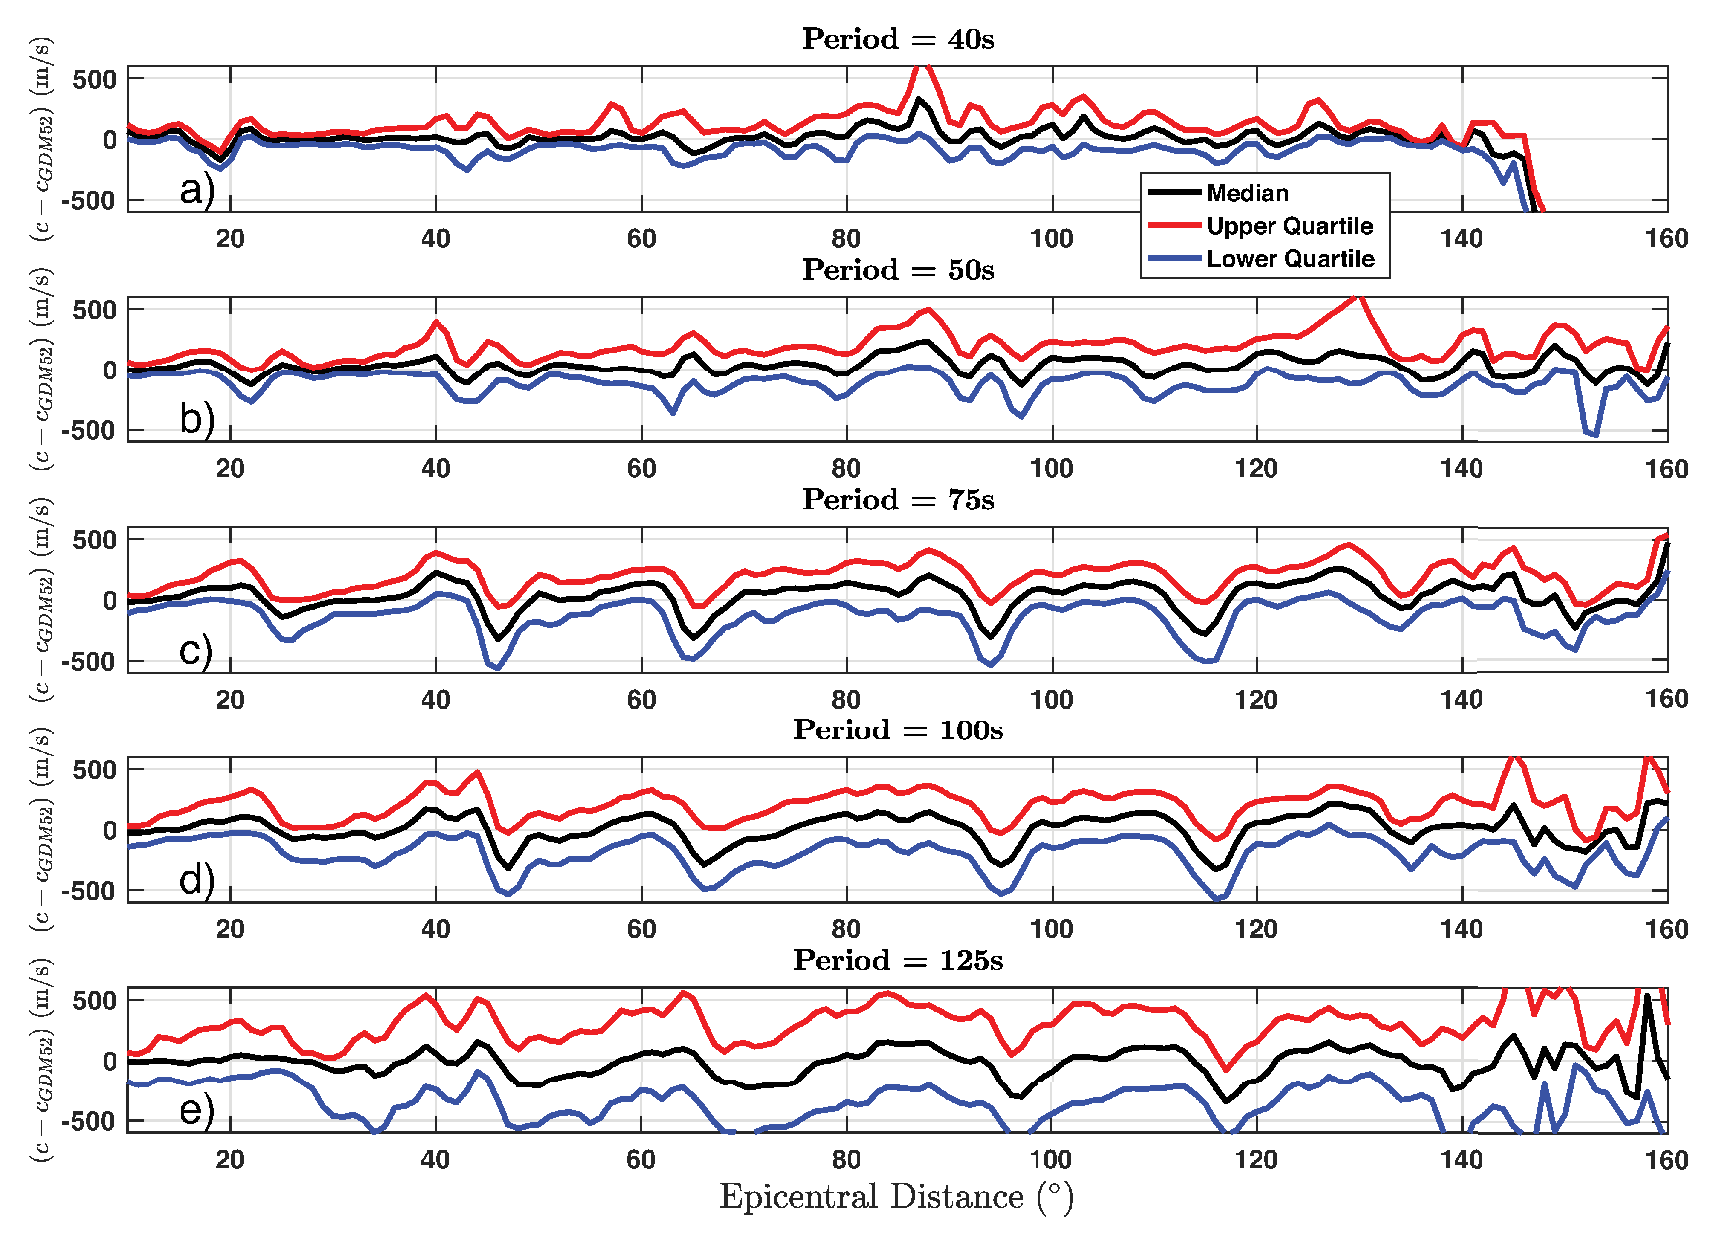
\includegraphics[width=0.99\textwidth]{Fig12_Sver.eps}
 \caption{Lower, middle, and upper quartile error in USArray Love wave Eikonal phase velocities, binned as a function of epicentral distance with bin width = $1^\circ$. Calculation of error is described in Section 4.}
\end{figure}

We then explore whether the excitation ratio exerts control on the Love wave errors. For every event in the data set, we calculate excitation for the FM and first overtone, using the STW105-C eigenfunctions if the event occurs beneath a continent and the ATL2a eigenfunctions otherwise. This associates every error estimate with an excitation ratio, and we bin error as a function of excitation ratio, using a bin width of $0.2^\circ$. Fig.\ 13 summarizes the median absolute value of binned error as a function of excitation ratio. The general trend is that error increases as excitation ratio increases. The correlation between error and excitation ratio suggests that when the source mechanism and depth poorly excite the FM and/or strongly excite the first overtone, measurements of the Love wave travel time are more likely to be biased. For array-based imaging methods that rely on differential travel times over short distances, these travel-time errors propagate into large phase-velocity errors \citep{foster2014overtone}. 

The correlation between error and excitation ratio also indicates that imposing quality control criteria based on excitation ratios may be a path forward to improving the quality of these data sets. Our USArray Love wave data were measured from earthquakes in the depth range 12-50 km. Some of these shallow events have large excitation ratios and correspondingly large phase-velocity errors (Fig.\ 13), and Fig.\ 3 hints that some events deeper than 50 km could have small excitation ratios and presumably small phase-velocity errors. Future work will explore whether making measurements on deeper events could increase the number of Love wave measurements with small excitation ratios and therefore small interference biases.

\begin{figure}
 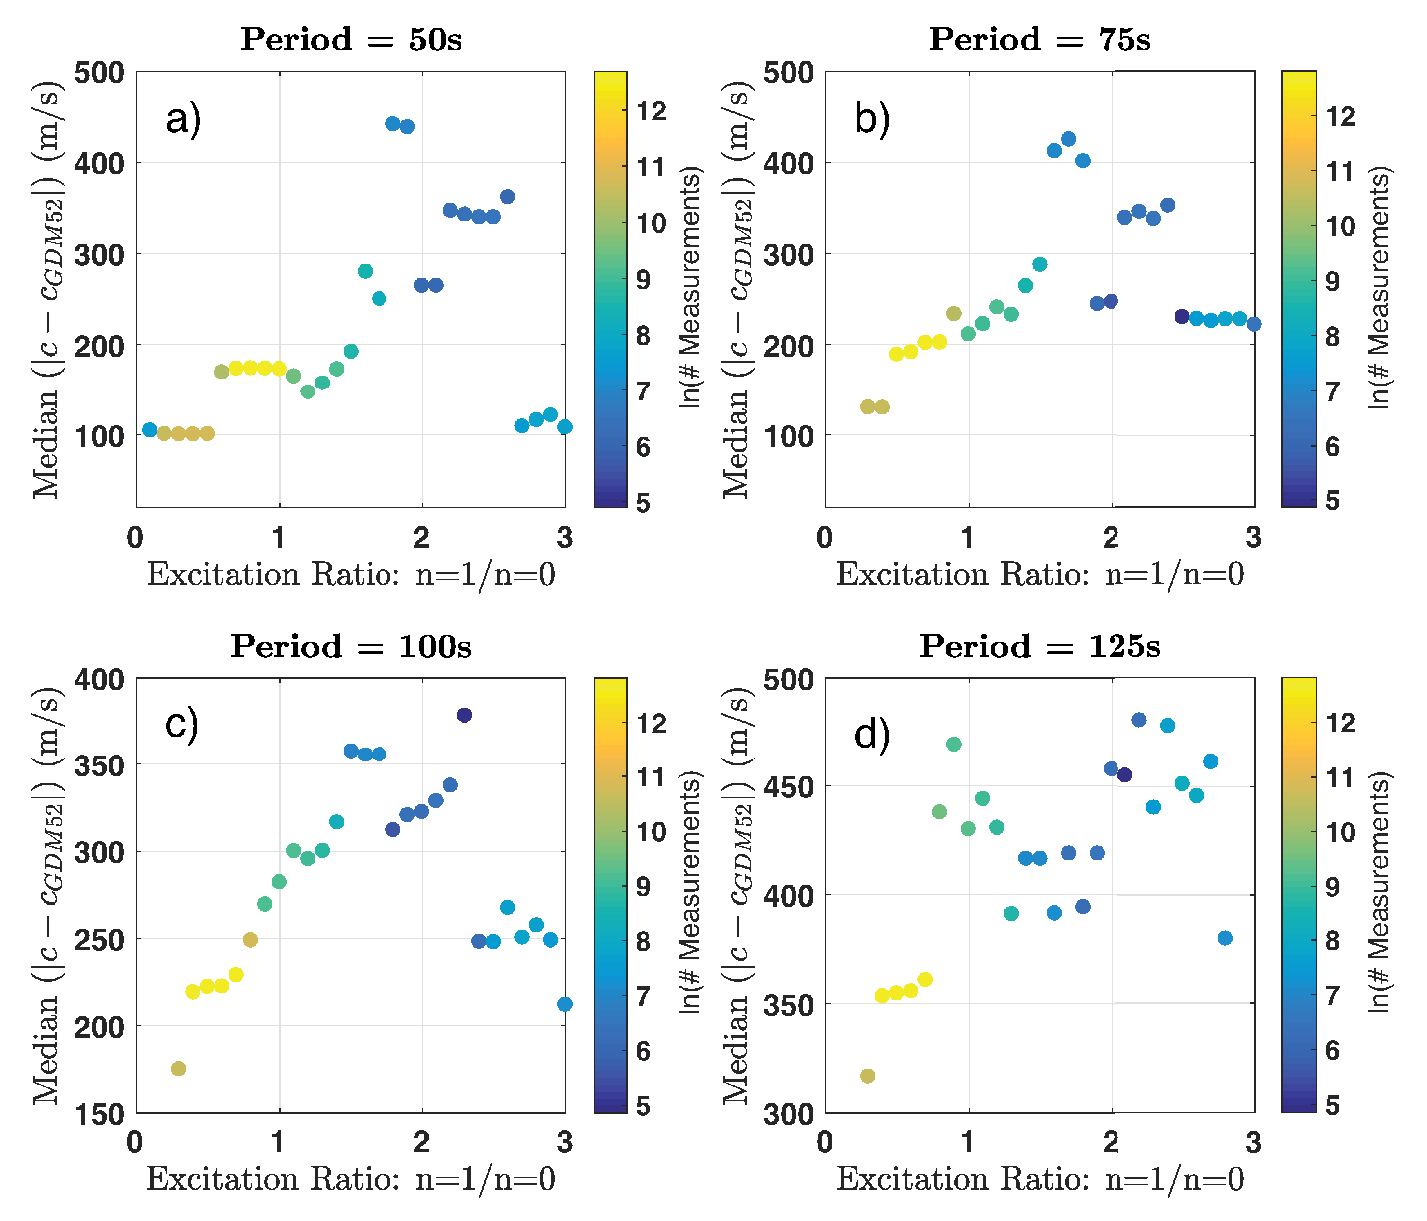
\includegraphics[width=0.99\textwidth]{Fig13_Sver.eps}
 \caption{Median absolute error in USArray Love wave Eikonal phase velocities, binned as a function of the ratio of the first-overtone excitation to the FM excitation. Color scale shows the number of measurements in each bin. }
\end{figure}
     
We have also found evidence in real Love wave data that overtones along the major arc interfere with the FM along the minor arc, as was suggested by our tests with synthetic seismograms. In Fig.\ 12, the wavelength of error decreases and the magnitude of error increases at large epicentral distances ($ \geq 140^\circ$). Fig.\ S9 shows that this major-arc interference can also be observed in event-specific phase velocity maps constructed from real data measured on USArray stations. In map view and in transect view, oscillations with a wavelength of approximately 3 degrees are clear. This wavelength is consistent with the prediction for major-arc interference (Equation 4) and much smaller than that expected for minor-arc interference ($\approx 18 ^\circ$ for Love waves at 75s, using phase velocities from STW105-C ) .     

Overall, our recommendation for event selection for Love wave is to calculate excitation ratios of the first overtone with respect to the FM for every event as a metric of measurement quality. Achieving a significant number of Love wave measurements with low excitation ratios will entail including measurements with source depths that are significantly larger than 50 km, particularly at longer periods. 


 \subsection{Rayleigh Wave Measurements on Real Data}

Fig.\ 14 summarizes the absolute value of the errors in USArray Rayleigh wave phase velocities, binned as a function of epicentral distance with bin width of 1$^\circ$. The dominant feature in these distributions of measurement error is the marked variation with distance, with a peak in error that is maximized at around 140$^\circ$, although the width and amplitude of this peak vary slightly between periods, with a larger and sharper peak at longer periods. At 100 s, the median error at 140$^\circ$ is larger by a factor of four than that at 60$^\circ$. Note that for this calculation, the phase velocity measurements shown at 120 s are differenced with the predictions from GDM52 at 125s, which is the closest period that exists in the GDM52 maps, while the measurements shown at other periods are differenced with predictions from the GDM52 map at exactly the same period. This slight mismatch of periods at 120 s does not appear to impact our conclusions.

\begin{figure}
\includegraphics[width=0.99\textwidth]{Fig14_Sver.eps}
\caption{Blue curve and left vertical axis: median absolute errors in USArray Rayleigh wave Eikonal phase velocities with respect to the GDM52 maps, binned as a function of distance. Red circles and right vertical axis: median excitation ratios for all events in the data set, labeled by overtone number $n$. The ratios show the excitation of overtone $n$ relative to the FM excitation and are plotted at the distance at which the overtone intersects the FM. }
\end{figure}

To show that the Rayleigh wave phase-velocity errors in Fig.\ 14 are controlled by the relative excitation of the overtones and FM, we calculate the excitation, using ATL2a, of the FM and first ten overtones for the source mechanism and depth and receiver location corresponding to every phase-velocity measurement in this data set. In Fig.\ 14 we show the median excitation ratio for each overtone relative to the FM for the entire data set, plotted at the distance where the overtone is predicted to intersect the FM. Overall, the variation of these median excitation ratios with distance mirrors the phase-velocity errors in real data and establishes that at distances $>$ 120$^\circ$, major-arc overtone interference is the dominant source of error. For example, at 100 s, the third overtone has the largest excitation ratio and intersects the FM at around 140$^\circ$, which is where the peak in phase-velocity error occurs. The ramp-up in error from 120$^\circ$ to 140$^\circ$ is reflected in the ascending excitation ratios of the overtones that intersect the FM in this distance range. At 50 s many of the excitation ratios are smaller than at 100 s, and their distribution is not as steeply peaked. This is mirrored in the smaller and less peaked phase-velocity errors.

Fig.\ 14 shows that the relative contribution of an overtone branch to the Rayleigh wave phase-velocity error depends on period. For example, at 100 s, the peak in error corresponds to the third overtone, but at 120 s it corresponds to the second and fourth overtones, with very small excitation of the third overtone, which corresponds to a Stoneley mode at 120 s. At 60 s, the peak corresponds to the fourth, fifth, and perhaps seventh overtones. This variation is entirely expected from the period dependence of the excitation functions in Fig.\ 7. The Eikonal phase-velocity maps, and thus the error, are determined from the same group of earthquakes at all periods, but the relative weight of overtone and FM excitation depends on period.

There are several reasons why we do not expect a perfect correlation between the measurement errors and excitation ratios. Firstly, there will be variation in the distance at which an overtone intersects the FM based on the specific propagation paths and path-averaged group velocities for each measurement. To explore the scope of this variation, we allowed for path-specific variation in FM group velocities (which may be broadly expected to vary more than overtone group velocities) and calculated the range of intersection distances for each overtone/FM pair using Equation 1; intersection distances tend to be close to predictions from a 1-D Earth model, with the largest deviations present at short periods such as 50s, which shows a standard deviation of $2^\circ$ in intersection distances across all pairs and a mean difference of approximately $3^\circ$ relative to the 1-D prediction. Secondly, condensing the excitation ratios for 581 events (on average) with a range of source mechanisms and depths into a single value for the entire data set is an over-simplification. We note also that the agreement between measurement errors and excitation ratios is weaker at distances greater than 160$^\circ$, where the major-arc FM interferes with the minor-arc FM \citep[e.g.][]{levshin2005minor},which is not accounted for with these excitation ratio calculations. Nonetheless, it is remarkable how well the observed errors can be explained by the combined effects of group velocity, which controls the intersection distance, and source excitation, which controls the strength of overtones and FM. 

\begin{figure}
 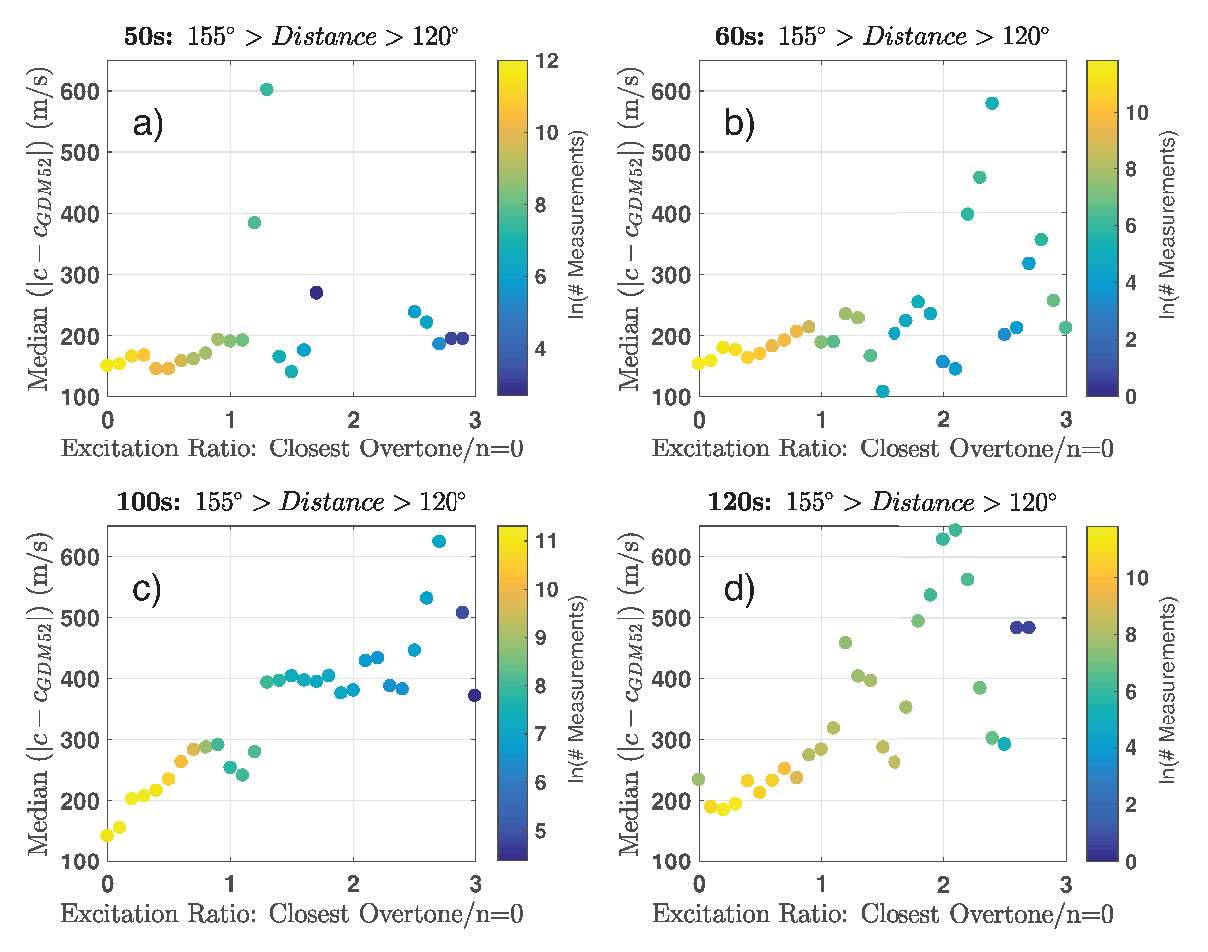
\includegraphics[width=0.99\textwidth]{Fig15_Sver.eps}
 \caption{Median absolute error in USArray Rayleigh wave Eikonal phase velocities in the distance range prone to major-arc interference, binned as a function of the ratio of closest overtone excitation to FM excitation. Color scale shows the number of measurements in each bin. The ``closest overtone'' is that that intersects the FM at the distance closest to each measurement; see text.}
\end{figure}

In Figs.\ 15 and 16 we bin Rayleigh wave phase-velocity error by excitation ratio rather than distance in the distance ranges most affected by major-arc and minor-arc interference, respectively. In the distance range of major-arc interference, each error measurement is binned based on the excitation of the overtone that intersects the FM at the epicentral distance closest to where the measurement is made. For example, at 100 s, the error measured in a pixel located 122$^\circ$ from the earthquake would be associated with the seventh overtone and therefore binned based on its excitation ratio. A strong correlation between excitation ratio and error is visible at the longer periods (Fig.\ 15c,d). This is important for two reasons. One, it further establishes that source excitation of the overtones and FM is the primary control on phase-velocity error. Two, it suggests that even in the distance range where major-arc overtone interference is prominent, there is a subset of measurements that are minimally affected by the interference and could be used. Excitation ratio could be a valuable and more nuanced criterion for quality control rather than a blanket recommendation to exclude all measurements at distances greater than 120 $^\circ$, which may substantially reduce the size of data sets for certain station locations \citep{hariharan2020evidence}. 

\begin{figure}
 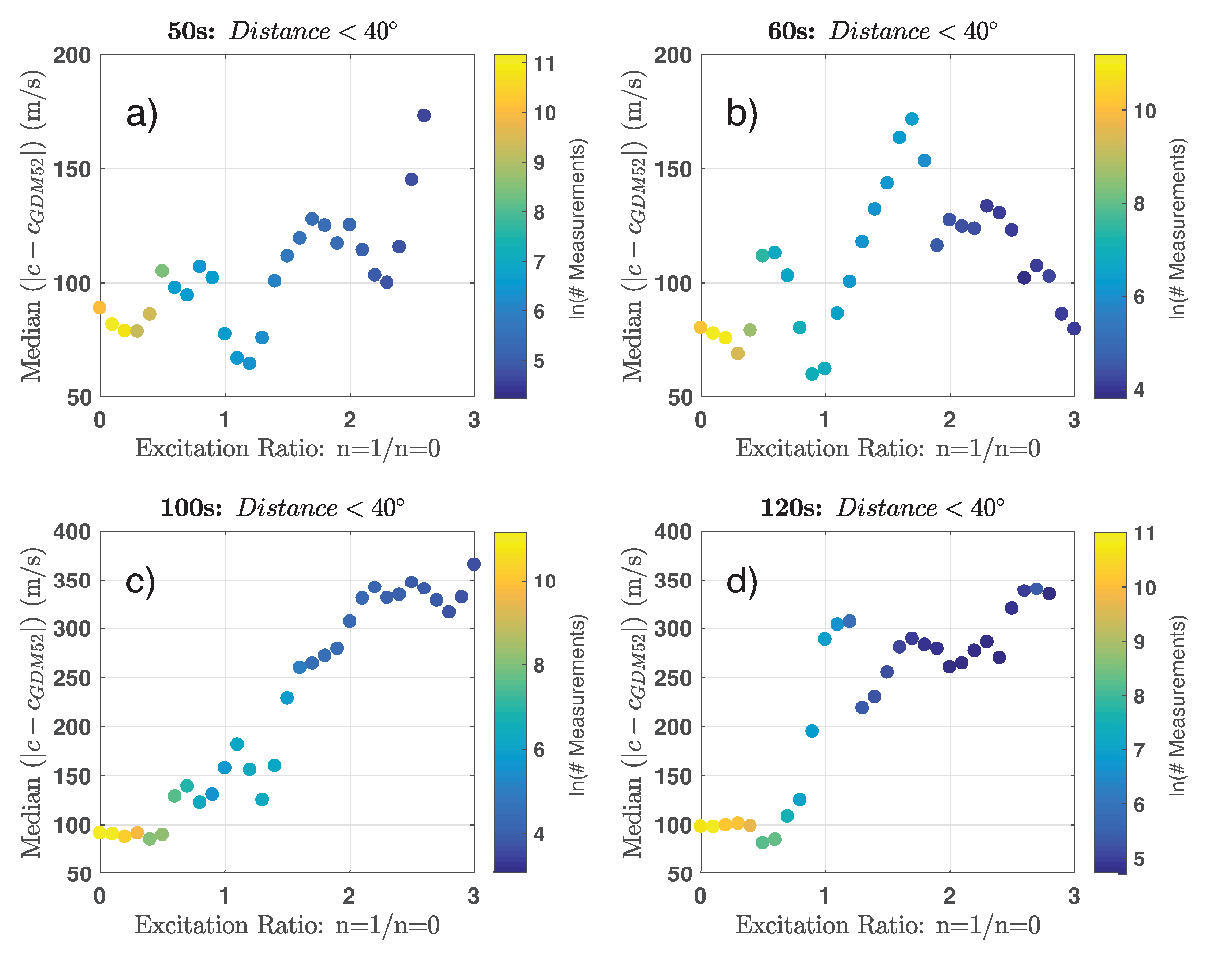
\includegraphics[width=1\textwidth]{Fig16_Sver.eps}
 \caption{Median absolute error in USArray Rayleigh wave Eikonal phase velocities in the distance range prone to minor-arc interference, binned as a function of the ratio of the first-overtone excitation to the FM excitation. Color scale shows the number of measurements in each bin.}
\end{figure}

Several factors may contribute to the weaker correlation observed at shorter periods in Fig.\ 15. These include path-dependent variability in the FM intersection distance for an overtone, as mentioned above, as well as the fact that Fig.\ 15 considers only the closest overtone when in some cases multiple overtones may be responsible for interference effects (Fig.\ 14). A third consideration is the impact of attenuation. The sensitivity of a surface wave to depth-dependent shear attenuation depends on overtone number \citep{dahlen1998theoretical}, which can result in different amounts of attenuation for different overtone branches, since shear attenuation varies with depth. Fig.\ S10d shows the impact of attenuation on the relative FM and overtone amplitudes. This calculation depends primarily on two factors: the attenuation ($Q^{-1}$) and intersection distance ($X$) for each overtone. The effect on surface-wave amplitude can then be calculated as $e^{\frac{-\omega X Q^{-1}}{2 U}}$, where $U$ is group velocity. At short periods, the high-$n$ overtones can experience much less attenuation (2-3 times less) than the FM. Thus, our assumption that source excitation ratio alone can control phase-velocity error is incomplete, because for the short-period high-$n$ overtones, the  excitation ratio is modulated by a ratio of the attenuation coefficient that can be of the same order of magnitude.

In the distance range of Rayleigh wave minor-arc interference, each error measurement is binned based on the excitation ratio of the first overtone to the FM (Fig.\ 16). As in Figs.\ 13 and 15, a strong correlation is visible, particularly at long periods. Minor-arc overtone interference for Rayleigh waves is typically considered negligible at epicentral distances $> 25^\circ$. However, the analysis in Fig.\ 16, as well as the interference patterns in Figs.\ 9 and 10, suggest that minor-arc interference may cause measurable bias up to longer distances. Although the majority of measurements are characterized by small excitation ratios, our analysis suggests that quality control at short to intermediate distances ( $ < 40^\circ$) based on excitation ratio would yield a cleaner data set. 

In the aforementioned analysis, we have used the Eikonal equation to solve for surface-wave phase velocities. While there are contemporary surface-wave imaging studies which only use the Eikonal equation to construct phase velocity maps \cite[e.g.][]{ball2016lithospheric,gama2021shear,lehujeur2020validity}, many studies instead use the Helmholtz equation \citep{lin2011helmholtz} to generate phase velocity maps \cite[e.g.][]{jin2015surface,babikoff2019long,adams2018relationships}. This is because Helmholtz phase velocities have been shown to better incorporate finite-frequency effects in phase velocity calculations \citep{lin2011helmholtz} than Eikonal velocities. It is thus worth considering the extent to which they are impacted by overtone interference. \citet{hariharan2020evidence} showed that Helmholtz phase velocities are still prone to overtone interference, but to a slightly reduced extent that for Eikonal velocities. To reinforce this point, we repeat the analysis in Figure 14, but for Helmholtz velocities at 100s. Figure S11 shows errors in both Helmholtz and Eikonal velocities, binned as a function of distance. As in the Eikonal case, errors in Helmholtz velocities increase sharply at epicentral distances greater than about 120 degrees, coincident with the large excitation ratios that correspond to overtones intersecting the FM arriving at these distances. However, the binned errors in Helmholtz phase velocities are slightly lower, reaching a maximum of approximately 270 m/s as opposed to 440 m/s for Eikonal phase velocities. However, the shape of the error distribution in Helmholtz velocities is similar to that of the Eikonal velocities- both cases begin to ramp up at the same  epicentral distance, and also reach their maxima at the same epicentral distance.

Overall, our analysis highlights the ability of excitation ratios to explain errors in inter-station Rayleigh wave phase velocity measurements. On average, these errors tend to be more pronounced at large epicentral distances due to more well-excited overtones arriving at these distances. Our recommendation is to consider the excitation ratios of overtones closest to the epicentral distance at which interstation phase-velocity measurements are made, and to use this as a measure of overtone contamination and measurement quality. We have shown that the paradigm that the most well-excited surface waves correspond to source depths shallower than 50 km is not always the case; we thus suggest that workers can consider including larger source depths in their datasets without issue, as long as the relevant excitation ratio is evaluated prior to measurement inclusion.

\section{Conclusion}
Using normal-mode synthetic seismograms calculated for 1-D Earth models, we illustrate the nature and diversity of overtone interference in FM Rayleigh wave and Love wave measurements of amplitude and travel time. We show that the strength of overtone interference on travel time and amplitude can span a wide range and varies strongly as a function of period and source mechanism and depth. Although the character of interference in Rayleigh and Love wave measurements is dramatically different, we show that in both cases it is controlled by the group velocities and source excitation of the overtones. We present excitation functions for the FM and first ten overtones for three example source mechanisms. For Rayleigh waves, we show that the distance at which an overtone intersects the FM and its excitation relative to the FM can explain the fine-scale features in travel-time and amplitude interference at both the scale of a single event and the distributions of error for an entire data set. For Love waves, we show that excitation ratio between the first overtone and fundamental mode is similarly correlated with the distribution of error in a regional data set, and that the Love wave data suffer from overtone interference along the major arc in addition to the minor arc.

We show that the error introduced by overtone interference into interstation (array-based) phase-velocity measurements depends on the magnitude of the travel-time bias, which is controlled by the relative excitation of an overtone and the closeness of its group velocity to the fundamental-mode group velocity, and the wavelength of the interference pattern, which is controlled by the phase velocities of the FM and overtone. Thus, the small-wavelength nature of major-arc interference can produce large errors in phase velocity. We note that overtone interference may impact other surface-wave observables and products. For example, regional measurements of attenuation, when made with an interstation approach such as the two-station method \citep{zhou2020rayleigh} or a wavefront-tracking approach \citep{xbaoattenuationsurfacewaves} may be vulnerable due to interference in amplitudes. Other examples of vulnerable observables are single-station (rather than path-averaged) quantities such as H/V ratios \citep{tanimoto2008zh} and site amplification \citep{eddy2014local,schardong2019anatomy}. 

Therefore, when possible, it is worth taking measures to avoid overtone interference. For measurements of the FM, we suggest quality control measures based on the relative excitation of overtones and the FM and, for Rayleigh waves at distances $>$ 120$^\circ$, the predicted intersection distances of overtones with the FM. Data selection by the source excitation ratio could also allow more nuanced choices, for example that Rayleigh wave measurements from certain events could be included if the period and distance range predicts little interference and excluded otherwise. Just as importantly, our calculations suggest that there is no reason to restrict all source depths in a data set to be shallower than 50 km  \citep[e.g.][]{jin2015crust,accardo2017surface,adams2018relationships,babikoff2019long}. This depth range includes some events with high overtone-to-FM excitation ratios, particularly at shorter periods for Rayleigh waves, and excludes deeper events with low excitation ratios, particularly for Love waves. Thus, such quality-control measures may allow for both the size and quality of typical surface-wave data sets to be increased. Considering the variations in overtone excitation ratio can also benefit studies aiming to extract overtone dispersion of a specific overtone; depending on the overtone targeted, event selection can be optimized to maximize the excitation ratio of the overtone of interest relative to other modes in the window.  A careful assessment of how different data selection strategies impact the size and quality of regional FM surface-wave data sets will be the subject of a future publication.  

\newpage 

\begin{acknowledgments}
We thank Ge Jin and an anonymous reviewer for constructive feedback that improved the quality of this manuscript. This work was supported by the U.S National Science Foundation under grants EAR-1553367 and EAR-1829401 and also by an NSF Graduate Research Fellowship under grant number DGE-16-44760. GMT software \citep{wessel1998new} was used for figure construction.
\end{acknowledgments}

\begin{dataavailability}
The seismic data from USArray used to make surface-wave measurements in this study can be downloaded from the IRIS DMC. Normal mode synthetic seismograms can be generated with the MINEOS code \citep{mineosbro}, which can be downloaded from CIG at https://geodynamics.org/cig/software/mineos/
\end{dataavailability}

\bibliographystyle{gji}
\bibliography{agusample.bib}


\label{lastpage}


\end{document}
